\documentclass[12pt,a4paper]{article}
\usepackage[a4paper,margin=3.5cm]{geometry}
\usepackage[utf8]{inputenc}
\usepackage[english]{babel}


% Citations and bibliography
\usepackage{natbib}
\bibliographystyle{abbrvnat}

% Table of contents and section headers
\setcounter{tocdepth}{2}
\setcounter{secnumdepth}{2}

% Enumerations
\usepackage{paralist}

% Graphics
\usepackage{xcolor}
\usepackage{graphicx}
\graphicspath{{Figures/}}

% Custom commands
\newcommand{\silvan}[1]{\textcolor{blue}{[#1]}}

% Math
\usepackage{amssymb}
\usepackage{mathtools}
\usepackage{bm}
\usepackage{fancyvrb} % for "\Verb" macro
% Relations between variables
\DeclareMathOperator*{\CI}{{\,\perp\mkern-12mu\perp\,}}
\DeclareMathOperator*{\nCI}{{\,\not\mkern-1mu\perp\mkern-12mu\perp\,}}
\DeclareMathOperator*{\SEP}{\perp}
\DeclareMathOperator*{\nSEP}{\not\perp}
\newcommand{\indep}[4]{{#1} \CI_{#4} {#2} \given {#3}}
\newcommand\dep[4]{{#1} \nCI_{#4} {#2} \given {#3}}
\newcommand\sep[4]{{#1} \SEP_{#4} {#2} \given {#3}}
\newcommand\con[4]{{#1} \nSEP_{#4} {#2} \given {#3}}
\newcommand{\dsep}[4]{{#1} \SEP_{#4}^d {#2} \given {#3}}
\newcommand{\dcon}[4]{{#1} \nSEP_{#4}^d {#2} \given {#3}}
\newcommand{\sigmasep}[4]{{#1} \SEP_{#4}^\sigma {#2} \given {#3}}
\newcommand{\sigmacon}[4]{{#1} \nSEP_{#4}^\sigma {#2} \given {#3}}
\newcommand{\Prb}{\mathbb{P}}
\newcommand{\marg}[1]{\mathrm{marg}_{#1}}
\newcommand{\intervene}{\mathrm{do}}
% Bold, cursive
\newcommand\B[1]{\bm{#1}}
\newcommand\C[1]{\mathcal{#1}}
\newcommand\BC[1]{\bm{\mathcal{#1}}}
% Arrows (oriented, star, circle)
\newcommand{\ot}{\leftarrow}
\newcommand{\oto}{\leftrightarrow}
\newcommand{\ots}{\leftarrow\mkern-13mu\ast\,}
\newcommand{\otc}{\leftarrow\mkern-9mu\circ\,}
\newcommand{\sto}{\,\ast\mkern-13mu\to}
\newcommand{\stt}{\,\ast\mkern-13mu\relbar\!\!\!\relbar}
\newcommand{\tts}{\relbar\!\!\!\relbar\mkern-13mu\ast\,}
\newcommand{\sts}{\,\ast\mkern-10mu\relbar\mkern-10mu\ast\,}
\newcommand{\ctc}{\,\circ\mkern-9mu\relbar\mkern-9mu\circ\,}
\newcommand{\cto}{\,\circ\mkern-9mu\rightarrow}
% Graph relations
\newcommand\mathbfsc[1]{\text{\normalfont\scshape#1}}
\newcommand\Det[1]{\mathbfsc{Det}(#1)}
\newcommand\an[1]{\mathbfsc{an}(#1)}
\newcommand\de[1]{\mathbfsc{de}(#1)}
\newcommand\scc[1]{\mathbfsc{sc}(#1)}
\newcommand\pa[1]{\mathbfsc{pa}(#1)}
\newcommand\ch[1]{\mathbfsc{ch}(#1)}
\newcommand\ncol[1]{\mathbfsc{ncol}(#1)}
\newcommand\col[1]{\mathbfsc{col}(#1)}
\newcommand\Detsub[2]{\mathbfsc{Det}_{#2}(#1)}
\newcommand\ansub[2]{\mathbfsc{an}_{#1}(#2)}
\newcommand\desub[2]{\mathbfsc{de}_{#1}(#2)}
\newcommand\sccsub[2]{\mathbfsc{sc}_{#1}(#2)}
\newcommand\pasub[2]{\mathbfsc{pa}_{#1}(#2)}
\newcommand\chsub[2]{\mathbfsc{ch}_{#1}(#2)}
% Names
\newcommand\mec{\mathbfsc{mec}}
% Other
\newcommand\given{\,|\,}


\begin{document}

\newgeometry{margin=2cm}

\begin{titlepage}



    \newcommand{\HRule}{\rule{\linewidth}{0.5mm}} % Defines a new command for the horizontal lines, change thickness here
    
    \center % Center everything on the page
    
     
    
    %----------------------------------------------------------------------------------------
    
    %	HEADING SECTIONS
    
    %----------------------------------------------------------------------------------------
    
    
    
    
\includegraphics[width=\linewidth]{uvalogo}\\[2.5cm]
    
    \textsc{\Large MSc Artificial Intelligence}\\[0.2cm]
    
    \textsc{\Large Master Thesis}\\[0.5cm] 
    
    
    
    %----------------------------------------------------------------------------------------
    
    %	TITLE SECTION
    
    %----------------------------------------------------------------------------------------
    
    
    
    \HRule \\[0.4cm]
    
    { \huge \bfseries Topology-Based Causal Analysis \\ and Gene Expression Data}\\[0.4cm] % Title of your document
    
    \HRule \\[0.5cm]
    
     
    
    %----------------------------------------------------------------------------------------
    
    %	AUTHOR SECTION
    
    %----------------------------------------------------------------------------------------
    
    
    
    by\\[0.2cm]
    
    \textsc{\Large Silvan de Boer}\\[0.2cm] %you name
    
    12158054\\[1cm]
    
    
    
    
    
    %----------------------------------------------------------------------------------------
    
    %	DATE SECTION
    
    %----------------------------------------------------------------------------------------
    
    
    
    {\Large \today}\\[1cm] % Date, change the \today to a set date if you want to be precise
    
    
    
    48 ECTS\\ %
    
    November 2019 - September 2020\\[1cm]%
    
    
    
    %----------------------------------------------------------------------------------------
    
    %	COMMITTEE SECTION
    
    %----------------------------------------------------------------------------------------
    
    
    \begin{minipage}[t]{0.4\textwidth}

    \begin{flushleft} \large
    
    \emph{Supervisor:} \\
    
    Prof J \textsc{Mooij} % Supervisor's Name
    
    \end{flushleft}
    
    \end{minipage}% 
    \begin{minipage}[t]{0.4\textwidth}
    
    \begin{flushright} \large
    
    \emph{Assessor:} \\
    
    Dr P  \textsc{Forr\'{e}}\\
    
    \end{flushright}
    
    \end{minipage}\\[2cm]
    
    
    %----------------------------------------------------------------------------------------
    
    %	LOGO SECTION
    
    %----------------------------------------------------------------------------------------
    
    
    
    % \framebox{\rule{0pt}{2.5cm}\rule{2.5cm}{0pt}}\\[0.5cm]
    
    
\includegraphics[width=2.5cm]{uvalogo2.png}\\ % Include a department/university logo - this will require the graphicx package
    
    \textsc{\large Informatics Institute}\\[1.0cm] % 
    
     
    
    %----------------------------------------------------------------------------------------
    
    
    
    \vfill % Fill the rest of the page with whitespace
    
    
    
    \end{titlepage}

    \restoregeometry

\newpage
\tableofcontents

\newpage
\section*{Notation and Terminology}

\begin{tabular}{lll}

$X, Y, Z$           & \verb.X.              & random variable, or a node representing it \\
$x, y, z$           & \verb.x.              & value of random variable $X, Y, Z$ \\
$X\to Y$            & \verb.\to.            & $X$ is a direct, or ancestral cause of $Y$ \\
$X\oto Y$           & \verb.\oto.           & $X$ and $Y$ are confounded \\
$\Prb_{\BC{X}}$     & \verb.\Prb_\BC{X}.    & probability measure on some (product) space \\
$p_{\B{X}}$         & \verb.\p_\B{X}.       & probability density (or: mass) function of $\Prb_{\BC{X}}$ \\
$\C{M}$             & \verb.\C{M}.          & structural causal model (SCM) \\
$\C{H}_{\C{M}}$,$\C{G}_{\C{M}}$ & \verb.$\C{H}_{\C{M}}$. & augmented graph resp. graph of some SCM \\



\end{tabular}

\section{Introduction}

% Causality: statistical + symbolic AI
\begin{frame}
    \frametitle{Artificial Intelligence}
    \begin{itemize}
        \item Statistical Artificial Intelligence
            \begin{itemize}
                \item Deduction
                \item Data
                \item Opaque
            \end{itemize}
        \item Symbolic Artificial Intelligence
            \begin{itemize}
                \item Induction
                \item Knowledge
                \item Interpretable
            \end{itemize}
    \end{itemize}
\end{frame}

\begin{frame}
    \frametitle{Statistical Artificial Intelligence}
    
    \only<1>{
        \twoimg{1introduction/stat1.png}{1introduction/stat1appl.jpg}
    }
    \only<2>{
        \twoimg{1introduction/stat2.png}{1introduction/stat2appl.jpeg}
    }
    \only<3>{
        \twoimg{1introduction/stat3.jpeg}{1introduction/stat3appl.png}
    }
\end{frame}

\begin{frame}
    \frametitle{Symbolic AI}
    
    \only<1>{
        \twoimg{1introduction/symb1}{1introduction/symb1appl}
    }
    \only<2>{
        \twoimg{1introduction/symb2}{1introduction/symb2appl}
    }
    \only<3>{
        \twoimg{1introduction/symb3}{1introduction/symb3appl}
    }
\end{frame}

% Questions answerable with causality (encoding causal assumptions)
\begin{frame}
    \frametitle{Causality}

    \only<1>{
        \twoimg{1introduction/joint_distr}{1introduction/rct}
    }

    \only<2-3>{
        \begin{columns}
            \begin{column}{0.4\textwidth}
                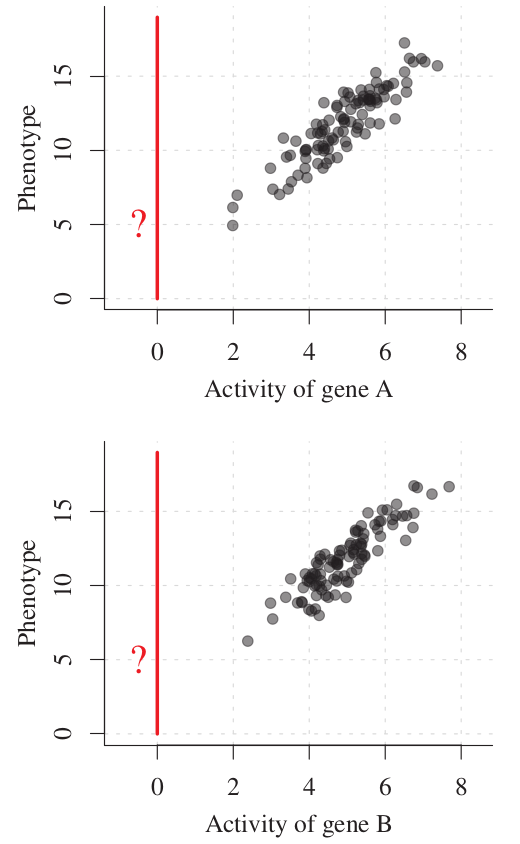
\includegraphics[width=\textwidth]{1introduction/causalknowledgeA.png}
            \end{column}
            \begin{column}{0.4\textwidth}
                \includegraphics<3>[width=\textwidth]{1introduction/causalknowledgeB.png}
            \end{column}
        \end{columns}
    }

    % Questions answerable by causality
    
    
    
\end{frame}




% Modeling causality: SCMs to encode causal assumptions (focus?: math or methods)


\begin{frame}
    \frametitle{Structural Causal Model}
    
\end{frame}


% Inspiration: Philips LCD (+ state-of-the-art)


% Aims and challenges



% 4 pages

\newpage
\section{Background}
\label{chapter:background}
% max 10 pages

\subsection{Modelling Framework}

\subsubsection{Structural Causal Model}
Throughout this thesis we will assume that the data is generated by a Structural Causal Model (SCM) $\C{M}$. This modelling framework is widely used in the field of causality, and is very flexible. 

A distinction is made between endogenous variables and exogenous variables. Endogenous variables are known, either by measurement (data $\B{X}$) or by design of some inference method (e.g. context variables $\B{C}$ in LCD). They are represented by an index set $\C{I}$. Exogenous variables are latent, a typical example is noise variables $\B{N}$. Exogenous variables are represented by an index set $\C{J}$.

The causal mechanism $\B{f}$ of a SCM is a function that describes how all variables relate to each other. It maps a product space of all variables to a product space of the endogenous variables. 

The components of the causal mechanism $f_i$ usually do not depend on all variables, but rather on a small subset that we call the parents of variable $X_i$. The augmented graph $\C{H}_{\C{M}}$ represents these child-parent relations with directed edges between variable nodes.

The exogenous variables are modelled with a product probability measure $\Prb_{\BC{E}}$, since their values are not measured. Data can then be sampled from a SCM by sampling from this measure and (iteratively) applying the functions $f_i$ to compute the values of the endogenous variables.

Usually, an incomplete definition of SCMs suffices, consisting of the structural equations of the endogenous variables and the density function of the exogenous variables, indicated below with $\B{X}$ and $\B{E}$ respectively:

$$\C{M}: \begin{cases}
    X_i &= f_i(\B{X}_{\pasub{}{i} \cap \C{I}}, \B{E}_{\pasub{}{i} \cap \C{J}}) \\
    p_{\B{E}} & = \prod_{j\in\C{J}} p_{E_j}
\end{cases}$$

In a practical setting we are unable to infer the real structure of the exogenous variables. A useful graphical representation of a SCM is the graph $\C{G}_{\C{M}}$, which is an abstraction of the augmented graph $\C{H}_{\C{M}}$. Only the endogenous variables are nodes in this graph. The relations among endogenous variables are still represented by directed edges ($i \to j$). Variables that are confounded by an exogenous variable (i.e. share an exogenous ancestor) are connected with a bidirected edge\footnote{The same representation of confounding is used when we marginalize over a subset of endogenous variables} ($i\oto j$).

\subsubsection{Causal Assumptions and Interventional Data}
If one observes two variables $X$ and $Y$, and measures a dependence among them, it is impossible to say if $X$ causes $Y$ or the other way around. More formally, one cannot infer the causal direction from a probability measure $\Prb_{\{X,Y\}}$ alone. This is why we have to rely on \textit{causal assumptions} \citep{pearl2009causality}. Some common assumptions are discussed in Section \ref{sec:back:prin}. Section \ref{sec:back:meth} describes inference methods that rely on these assumptions. 

One assumption particularly relevant to this thesis is related to the method of data acquisition. A distinction is made between \textit{observational data} and \textit{interventional data}. Observational data is gathered without interference with the system. We assume that there is an underlying SCM, and every data point is a sample from it. The sampling distribution approximates the observational distribution $\Prb_{\B{X}}$. It is theoretically impossible to infer any causal statements without further assumptions. 

Interventional data is gathered while we interfere with the system. Every data point is measured while an \textit{intervention} is performed. Formally, this intervention is modelled as a manipulation of the causal mechanism $\B{f}$ subject to some constraints or assumptions. This may render the causal inference problem theoretically possible. 

A concrete example is the \textit{perfect intervention}. A perfect intervention sets a variable $X_i$ to a fixed value $\xi_i$, denoted as $\intervene(X_i=\xi_i)$. This removes all the dependence of $X_i$ on its parents $\pasub{\C{H}}{i}$. The adapted SCM induces a different, interventional distribution $\Prb_{\B{X}|\intervene(X_i=\xi_i)}$. \citet{pearl2009causality} developed a do-calculus that can be used to make causal inferences from observational and intervenional data. As a simple example, take a system of two variables that are related as $X\to Y$. From the observational data we only know that $X$ and $Y$ are dependent. However, if we have access to distributions $\Prb_{\{X,Y\}|\intervene(X=x)}$ and $\Prb_{\{X,Y\}|\intervene(Y=y)}$ we can see that intervening on $Y$ does not affect $X$, whereas intervening on $X$ does affect $Y$. We conclude that $X$ causes $Y$. 


\subsubsection{Markov Property}
The Markov Property is a very common assumption that links the SCM to conditional independence relations (CIRs) in the data. The property follows from the definition of the SCM, so it does not add a restriction to our modelling. 

The notion of \textit{d-separation} is used to infer CIRs. We say that two variables $X$ and $Y$ are d-separated by a conditioning set of variables $\B{C}$, if all walks from $X$ to $Y$ are d-blocked by $\B{C}$. This is denoted as $\dsep{X}{Y}{\B{C}}{\C{G}}$. On each walk we will consider if the variables are a \textit{collider}, that is: if the adjacent edges of the walk point towards it ($...\to Z \ot ...$). A walk is \textit{d-blocked} in three cases:

\begin{compactenum}
    \item $X$ or $Y$ are in $\B{C}$
    \item The walk contains a non-collider $Z$ that is in $\B{C}$
    \item The walk contains a collider $Z$ that is not in $\B{C}$, nor any of the descendents of $\B{C}$
\end{compactenum}

Consider the graph in Figure \ref{fig:2:dsep}. By case 1, $X_1$ blocks the walk from $X_1$ to $X_3$. $X_2$ blocks this walk if it is in the conditioning set $\B{C}$ by case 2. According to case 3, the walk from $X_2$ to $X_4$ is blocked if neither $X_3$ nor $X_5$ are in $\B{C}$.

\begin{figure}[h]
    \centering
    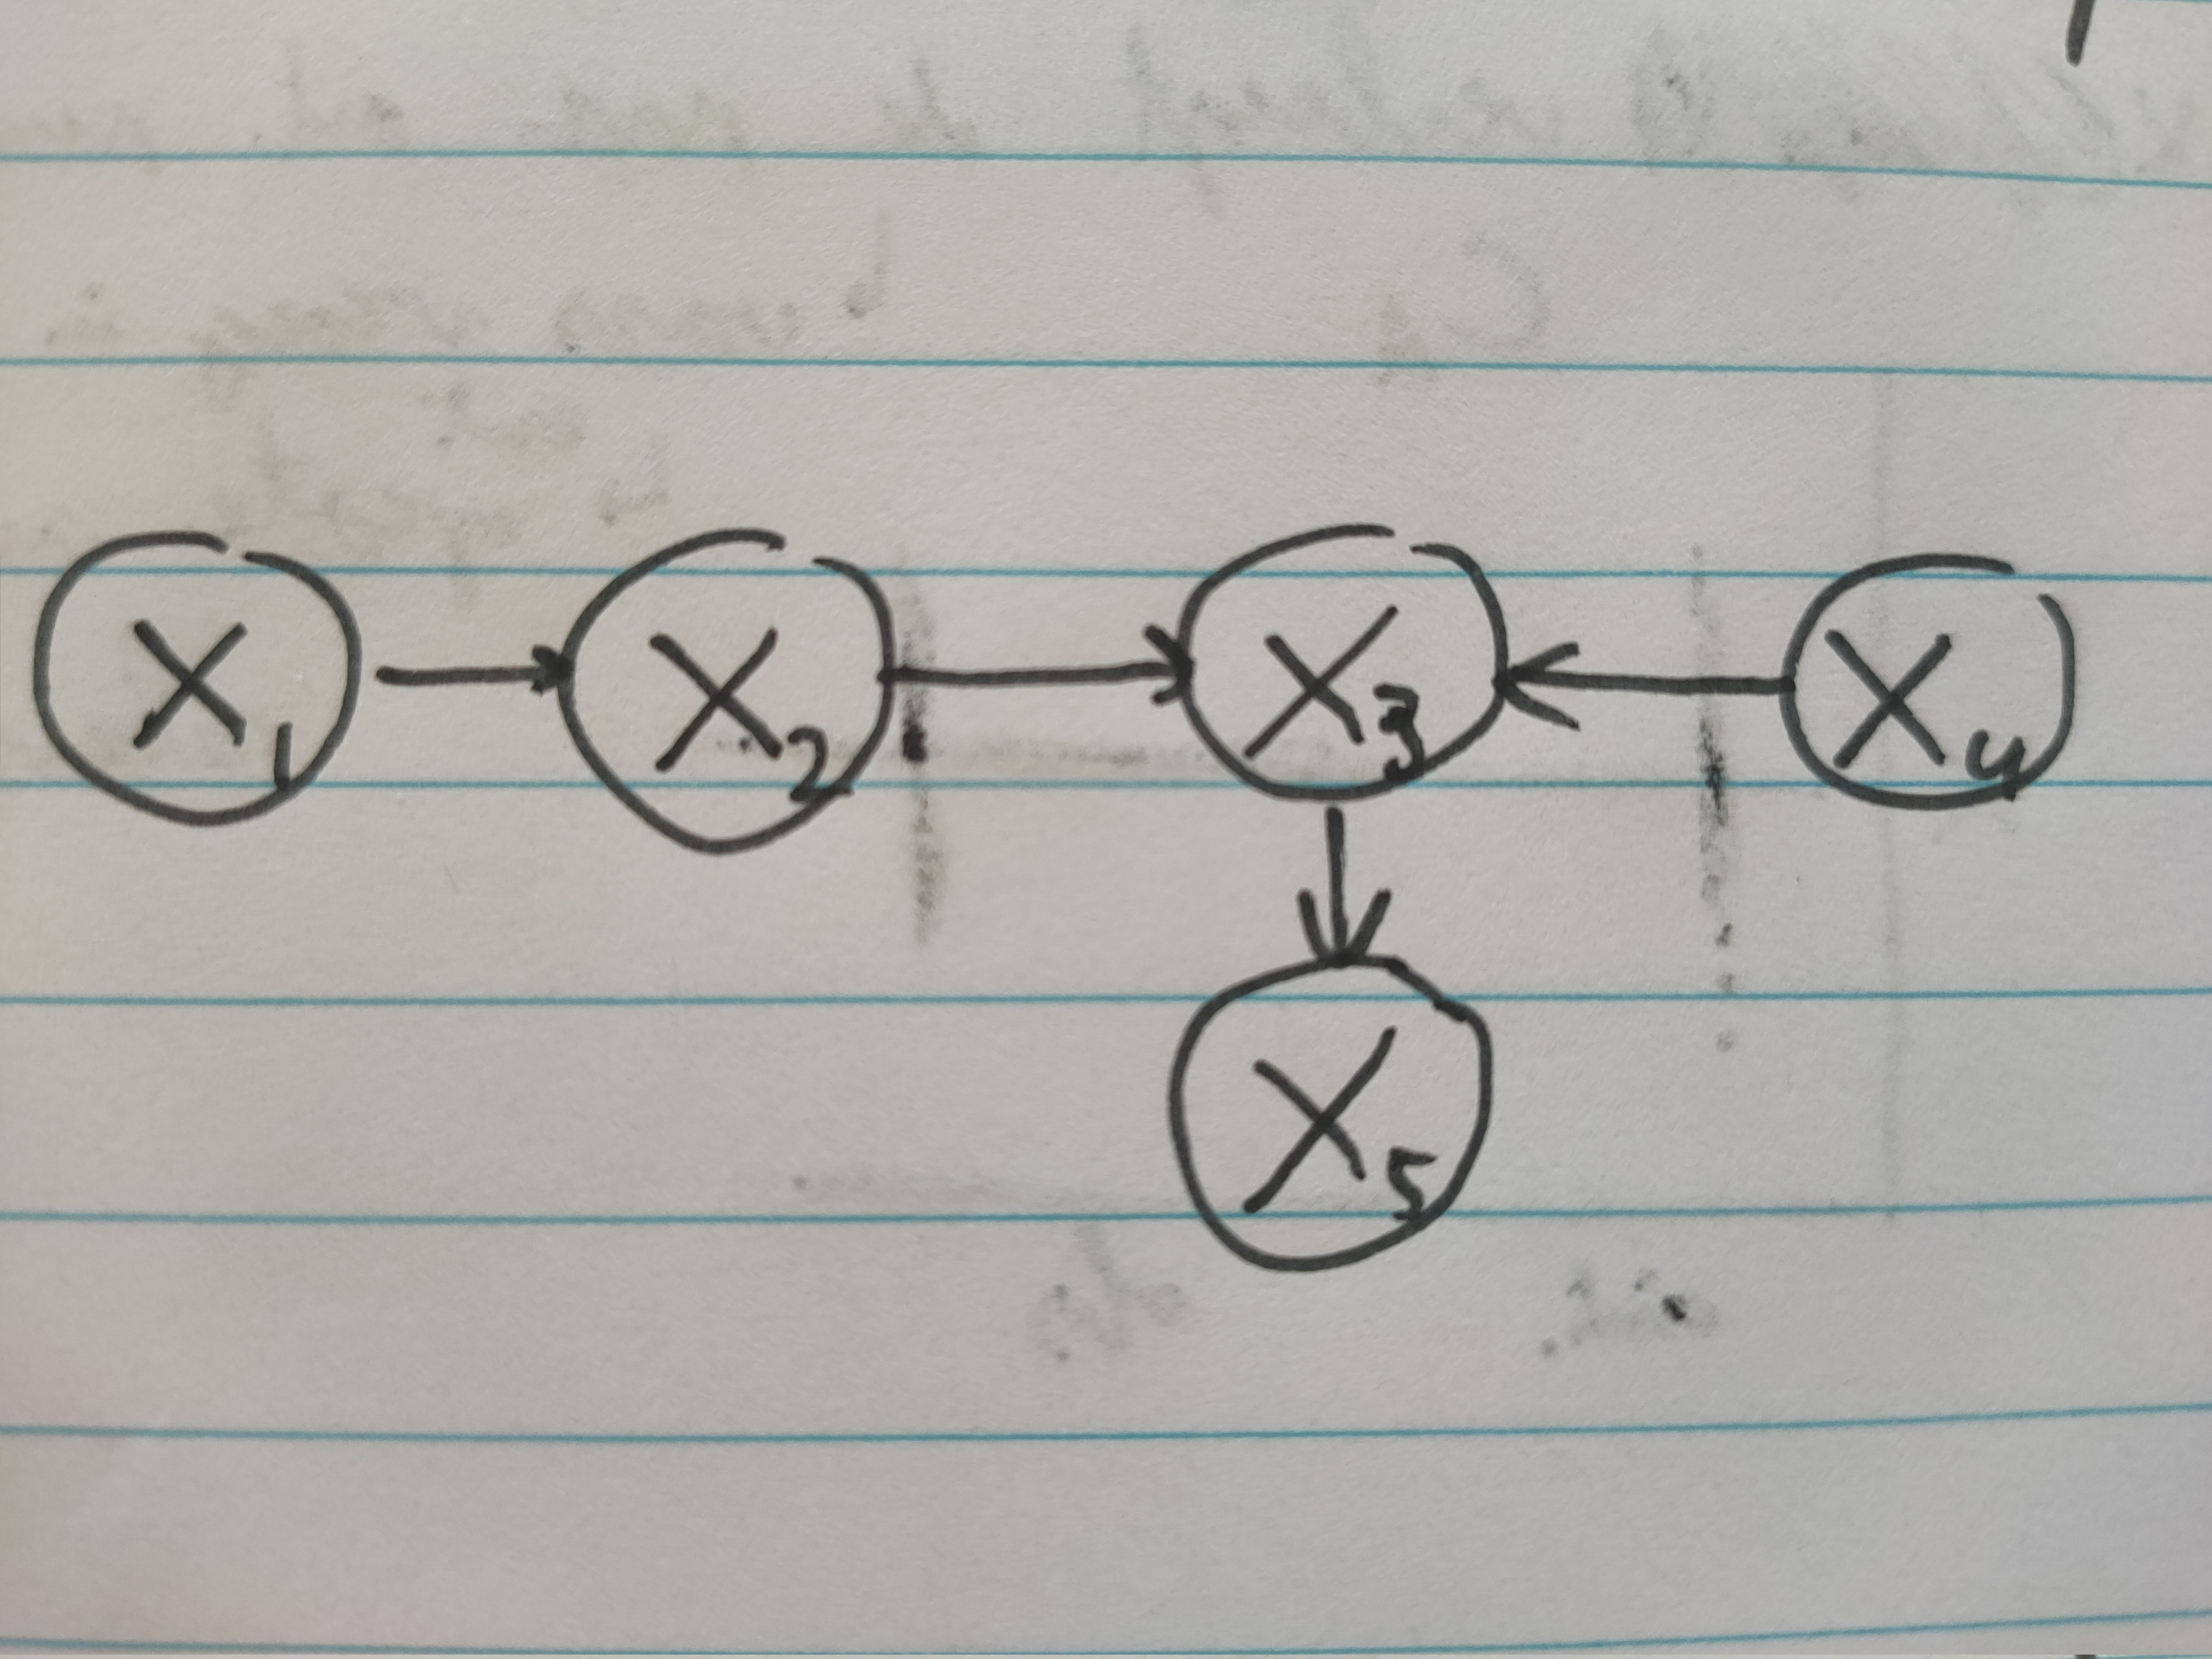
\includegraphics[width=\textwidth]{2dsep}
    \caption{Graph of five random variables.}
    \label{fig:2:dsep}
\end{figure}

The Global Markov Property links d-separation to conditional independence:

$$\dsep{\B{A}}{\B{B}}{\B{C}}{\C{G}} \implies \indep{\B{A}}{\B{B}}{\B{C}}{\Prb_{\B{X}}}$$

The Markov Property with d-separation is only valid for SCMs with an acyclic graph\footnote{It is also valid for some restricted cases of cyclic SCMs, cf. \citet{forre2017markov}}. A generalization of d-separation was developed by \citet{forre2017markov} that applies to the cyclic case as well.

Different graphs may satisfy the same set of d-separations. Therefore, some observational distribution $\Prb_{\B{X}}$ may satisfy the Global Markov Property with respect to different graphs. The set of graphs that induces the same observational distribution\footnote{Formally, one graph may induce multiple distributions, and the MEC consists of graphs that induce the same distributions} as some graph $\C{G}$ is called its Markov Equivalence Class $\mec(\C{G})$. For acyclic graphs, it is shown that two graphs are equivalent if they have the same skeleton and immortalities \citep{verma1991equivalence}. The skeleton is the set of edges when we disregard their direction, an immortality is a local structure $A\to B \ot C$ in which $A$ and $C$ are not directly connected.

Causal inference methods that use only observational data cannot infer more than the MEC of the graph, because this is all the information that is in the observational distribution $\Prb_{\B{X}}$.


\subsubsection{Causal Inference Tasks}
Different tasks can be distinguished within causal inference. In this thesis we focus on methods that infer parts of the augmented graph $\C{H}$. These methods are not directly used to infer quantitative causal effects. However, the do-calculus of \citet{pearl2009causality} can in many cases be used to combine measured conditional distributions and a (partially) infered graph to make quantitative statements.

Generally, we can distinguish between global and local inference methods. Global methods aim to infer as much as possible from graph $\C{G}$. If the data is observational, these methods infer (an instance of) the MEC. An example is Inductive Causation, which naively checks the CIRs among all combinations of variables to infer the MEC. Interventional data enables some methods to infer more features of the graph. 

Local methods are specialized to find only some elements of the graph, usually trading completeness for efficiency. Commonly, these methods find some direct or ancestral causal relations (directed paths in $\C{G}$), like Local Causal Discovery which tests for one specific pattern of CIRs among three variables.


\subsection{Principles of Causal Inference}
\label{sec:back:prin}

\begin{figure}[h]
    \centering
    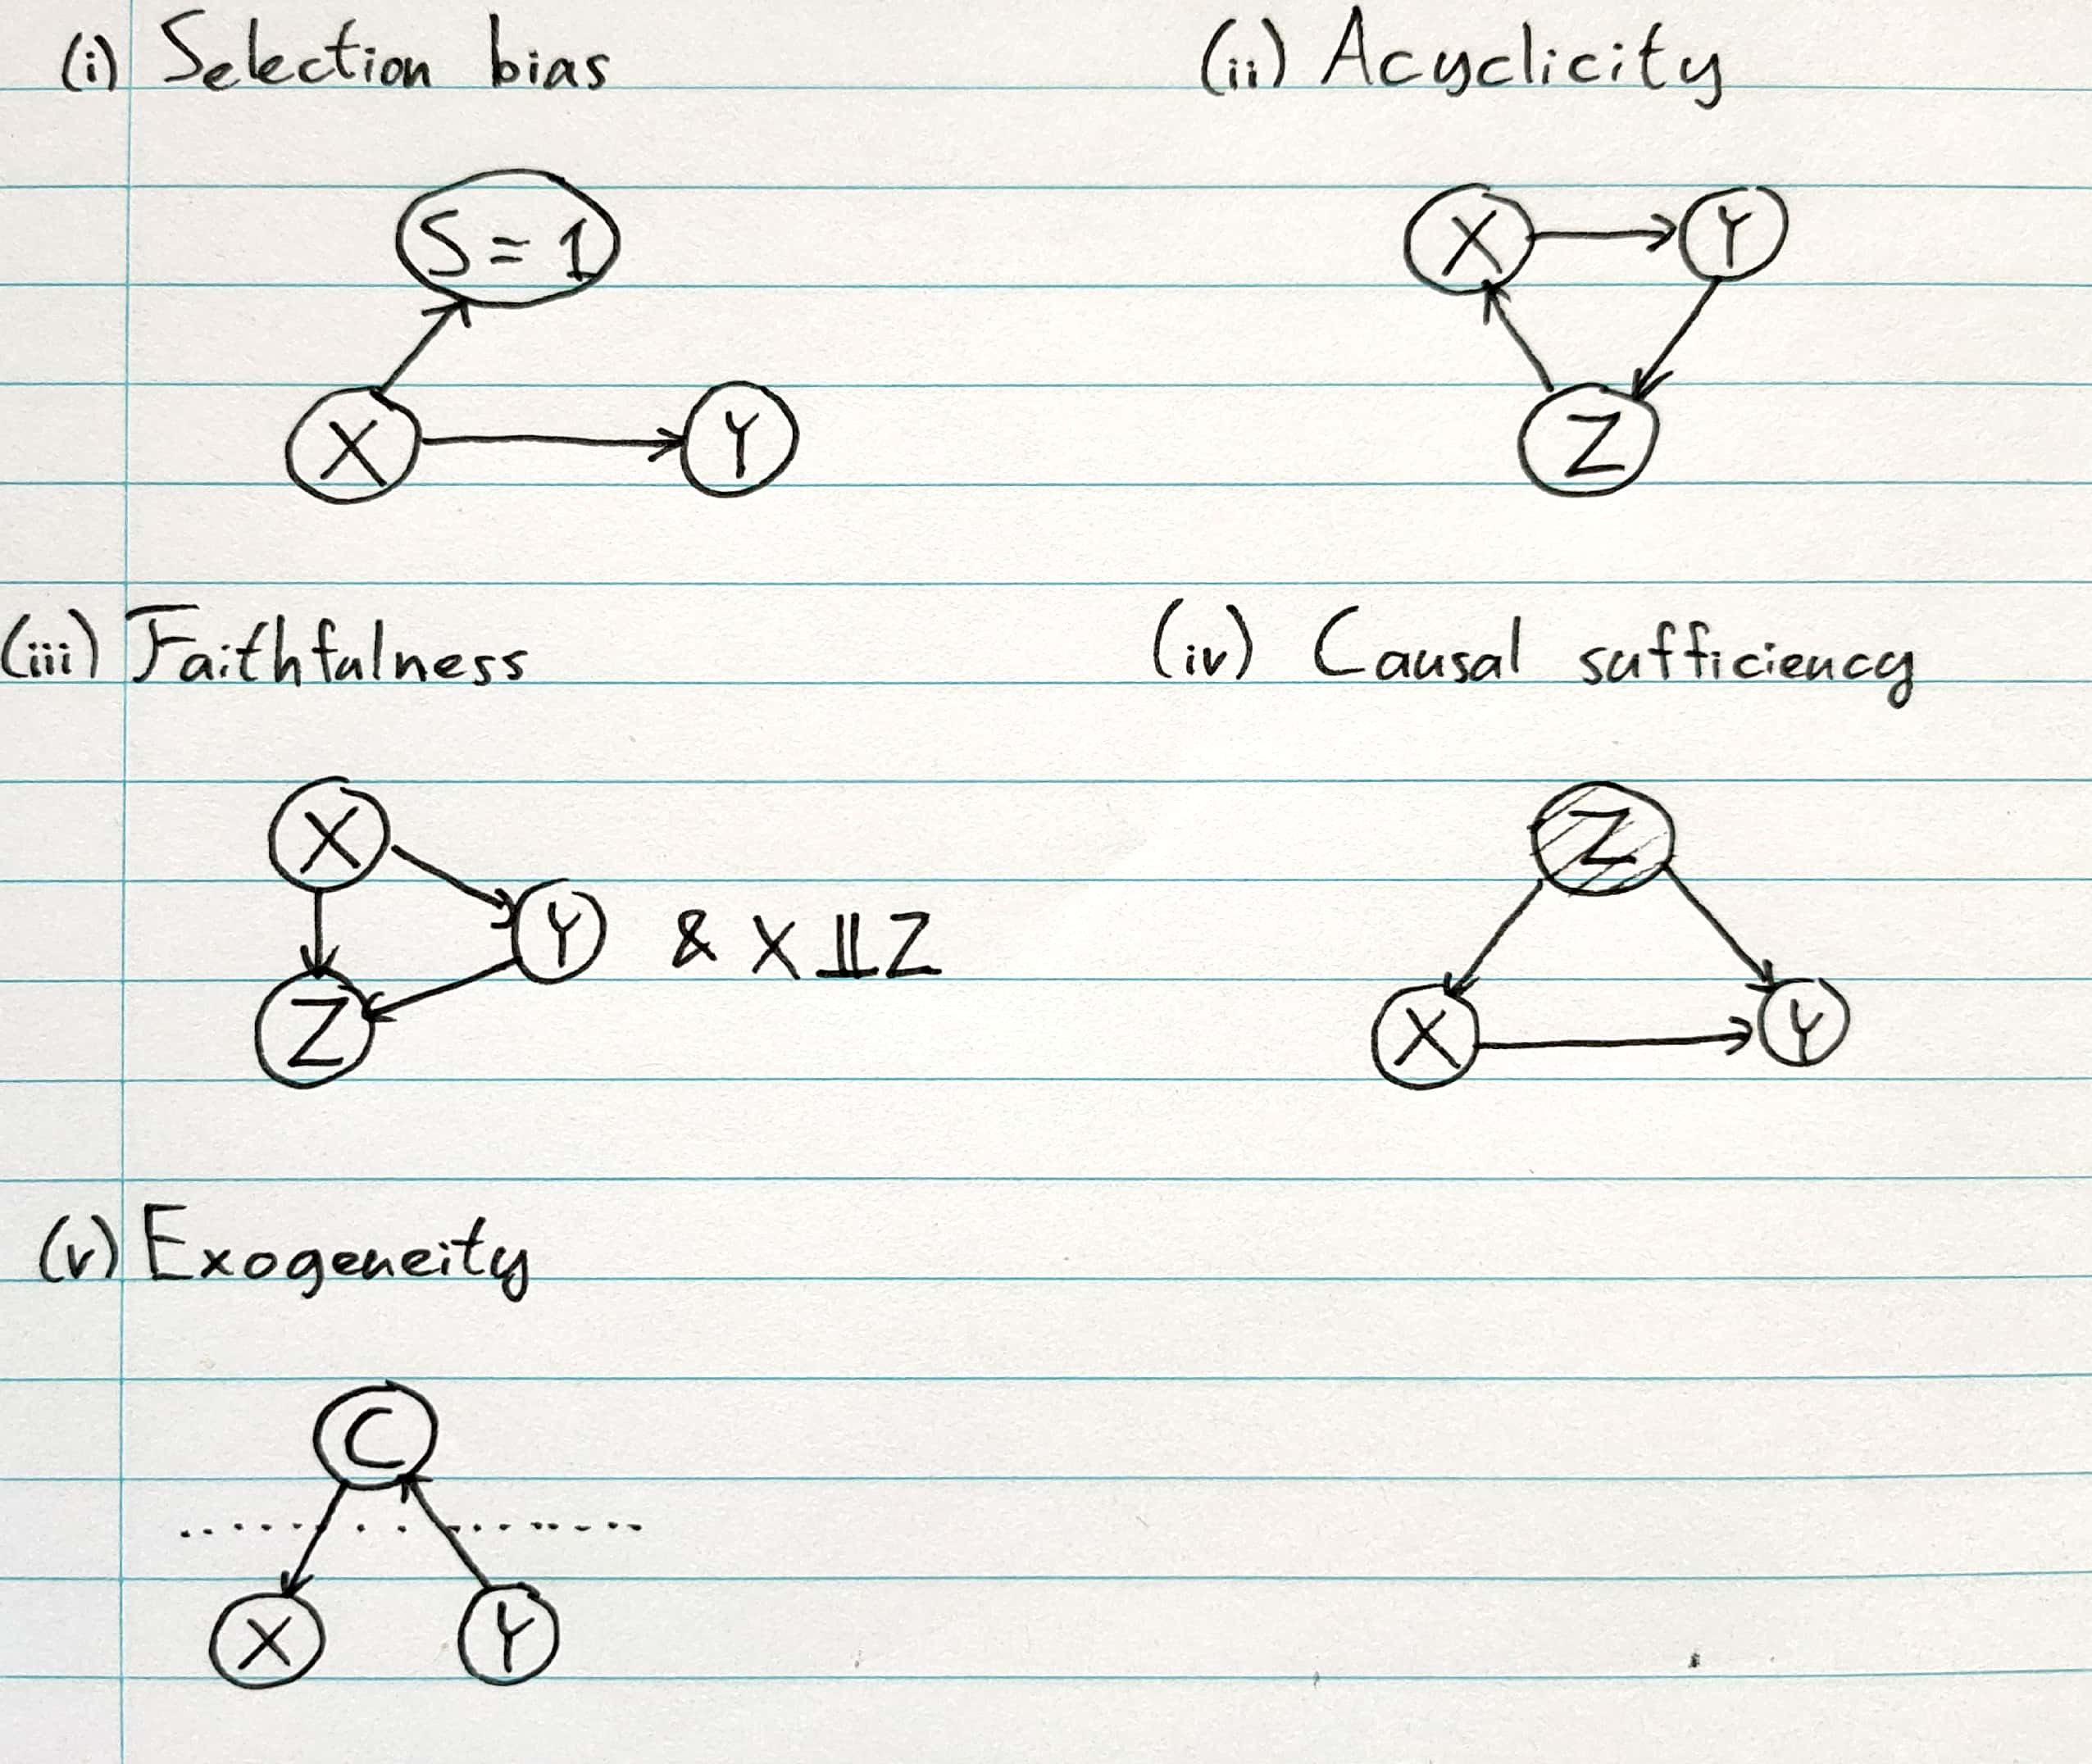
\includegraphics[width=\textwidth]{2assumptions}
    \caption{Violations of causal assumptions indicated by orange nodes or edges. Violation of faithfulness (iii) depends on the functional dependence between the variables, for example if $X \CI Z$}
    \label{fig:2:ass}
\end{figure}

Now that the general modelling framework of the SCM is established, it is time to define the most important additional assumptions that enable many causal inference methods. These assumptions are generally restrictions on the SCM.

\subsubsection{Reichenbach's common cause principle}

An important insight in causal inference is Reichenbach's common cause principle \citep{reichenbach1956direction}. It states that correlation is always the result of some causation. When two variables correlate, either one causes the other, or there is a third variable causing both. 

This is quite a strong assumption. It relies on i.i.d. sampling of the data, and a good approximation of the probability distribution. One should be cautious for spurious correlations. These can result from a search over correlations between many variables (without type I error control), or from overseeing a time dependence of the variables (violation of i.i.d. assumption). 

Moreover, the principle relies on the important assumption of \textbf{unbiased data selection}. Selection bias can be present when data selection is based on the value of some unobserved variable that is the effect of some observed variables. Take for example the graph in Figure \ref{fig:2:ass}i. The dependence between $X$ and $Y$ might disappear if we only consider data points for which $S=1$. 

This assumption is required for many causal inference methods. Take for example Local Causal Discovery (LCD), which depends on some local pattern of CIRs to infer an ancestral relation. If CIRs can be the result of selection bias, the pattern is not sufficient anymore to infer the ancestral relation.


\subsubsection{Faithfulness}

\textbf{Faithfulness} is a very common assumption. It reverses the implication of the Markov Property, such that conditional independence implies d-separation in the graph:

$$\indep{\B{A}}{\B{B}}{\B{C}}{\Prb_{\B{X}}} \implies \dsep{\B{A}}{\B{B}}{\B{C}}{\C{G}}$$

Many causal inference methods use this assumption to restrict the graph by measuring conditional dependences and independences. The test used to measure dependences and independences relies on additional assumptions, which we jointly call the assumption of an \textbf{independence oracle}. For example, the partial correlation test relies on normality of the data. When the data and assumptions are sufficient to infer the MEC of the graph, we say that the MEC is \textbf{identifiable}.

Faithfulness may be violated. Take the graph in Figure \ref{fig:2:ass}iii. Some causal mechanism may result in an independence between $X$ and $Z$, even though $Z$ is functionally dependent on $X$ and an intervention on $Y$ would show this.

Furthermore, faithfulness requires that all CIRs in the data are in the graph, which can be problematic. Especially when the graph is large and contains cycles, there may be hypothesis testing errors \citep{uhler2013geometry}.

% \silvan{ADD: Conditional independence testing has been proven to be impossible when no additional assumptions are imposed on the distributions involved (Shah and Peters, 2019) [P. Boeken]}

An implication of faithfulness is \textbf{causal minimality}. A distribution satisfies causal minimalty with respect to some graph if it is faithful to the graph, but not to any proper subgraph. 

One method that relies on faithfulness is Accounting for Strong Dependences (ASD). All dependence and independence relations are encoded as soft constraints in an Answer Set Programming (ASP) solver, along with constraints that determine how CIRs relate to the graph structure.

\subsubsection{Causal sufficiency}

The presence of latent (unobserved) variables can make it harder to identify parts of SCMs. Latent confounders that affect multiple variables influence the CIRs. Some methods rely on the assumption that there are no latent confounders: \textbf{causal sufficiency}. Figure \ref{fig:2:ass}iv shows a violation of this assumption, where $Z$ is latent.

Inductive Causation (IC) checks for every pair of variables $X$ and $Y$ that are dependent if there is a set of variables $\B{S}$ that renders them conditionally independent: $\indep{X}{Y}{\B{S}}{}$. If no such set exists, there must be a direct causal relation, because by Reichenbach's principle there cannot be another way in which they are dependent.

\subsubsection{Acyclicity}

The \textbf{acyclicity} assumption restricts the class of graphs to directed acyclic graphs (DAGs). Inference under this assumption is typically easier, because the class of possible graphs is much smaller. Nevertheless, some methods can be generalized when the concept of $\sigma$-separation is introduced to replace d-separation. 

One advantage of assuming acyclicity is that it is possible to define some ordering in the variables. In this order, variables precede their descendents in the graph. Greedy Equivalence Search (GES) is an example of a method that exploits this property. The search for the MEC is transformed to a search for an order that corresponds to the MEC. A greedy search algorithm is used to move between permutations of the order to efficiently find the correct MEC. 

\subsubsection{Exogeneity}

Some methods distinguish between two types of endogenous variables: the system variables $\B{X}$ and the context variables $\B{C}$. The context is seen as external to the system. This means that according to the \textbf{exogeneity}\footnote{Note that exogenous might refer to observed, endogenous context variables, or unobserved exogenous variables as represented by $\C{H}$} assumption, no edges in the graph can point from a system variable to a context variable. 

This assumption is violated in the graph in Figure \ref{fig:2:ass}v. We observe an effect on $X$ when we intervene on $Y$. If we assume that $C$ is exogenous, we could erroneously conclude that there is a direct relation $Y\to X$. In this case however, $C$ mediates this relation.

Typically, the context variables are used by the modeller to encode some causal background knowledge, such as the type of intervention. Invariant Causal Prediction (ICP) leverages the exogeneity assumption to compare the conditional distribution of a variable given a set of potential parents, accross values of the context. If the context itself is not a direct parent of the variable, this conditional distribution should be invariant, which allows ICP to infer causal relations. 

\subsection{Causal Discovery Methods}


\subsubsection{Constraint-Based Causal Discovery}
Constraint-based approaches derive constraints from the data, and use it to restrict the class of possible underlying causal graphs. Causal inference is treated as a constraint-satisfaction problem. Generally, conditional independence relations (CIR) are chosen as constraints, which can be used to derive the separation of variables and the orientation of edges in the graph. Some prominent methods are described below.

\textbf{Inductive Causation} (IC) was introduced by \citet{verma1991equivalence} and generally describes how we can induce a PDAG from conditional independences in the data. The algorithm consists of two steps: inducing the skeleton and orienting the edges. For every pair of variables $a$ and $b$, we check whether there is an edge in the PDAG. Using the faithfulness assumption, we add an edge if there is no separating set of variables $S_{ab}$ that makes $a$ and $b$ conditionally independent ($\nexists S : \indep{a}{b}{S_{ab}}{}$). One easy step of edge orientation uses the separation criterion of colliders. If two non-adjacent variables $a$ and $b$ share a neighbour $c$ that is not in $S_{ab}$, it must be a collider on the path and we induce edge orientation $a\to c \ot b$. Application of additional orientation rules lead us to a maximally oriented PDAG, which describes the Markov equivalence class of all causal graphs that induce the joint data distribution. One early set of such rules was described by \citet{spirtes2000causation} in the SGS algorithm, which was named after the authors.
            
IC is quite limited, because it relies on several assumptions about the underlying SCM (e.g. causal sufficiency), and its naive implementation is costly due to the search over all separating sets $S_{ab}$.

\textbf{PC}, named after its inventers Peter Spirtes and Clark Glymour \citep{spirtes1991algorithm}, reduces the cost of naive IC. A systematic algorithm finds the separating sets $S_{ab}$ in polynomial time. Starting from a fully-connected graph, edges are systematically removed by considering separating sets of increasing cardinality, and only taking into account the variables that neighbour $a$ and $b$. For example, first edges are removed between variable pairs that are independent given the empty set (cardinality 0). Then, edges are removed between remaining adjacent variable pairs that are independent given one of their neighbours. Already some possible separating sets can be skipped here, because edges were removed in the previous step. Therefore, as we consider larger possible separating sets, the number of neighbours to choose from decreases.
            
\textbf{Fast Causal Inference} (FCI) extends PC to allow for selection bias and latent confounding. Dropping the causal sufficiency assumption, means that it should consider some possible separating sets $S_{ab}$ that contain variables not adjacent to $a$ or $b$ (specifically, their ancestors). FCI is a feasible algorithm for datasets with many variables when the underlying graph is sparse and bidirected edges are not too much chained together. It was first introduced by \citet{spirtes1999algorithm}, and gradually developed since then. A modern version named FCI+ by \citet{claassen2013learning} is relatively fast. It finds the complete PAG in polynomial time.
            
\textbf{Invariant Causal Prediction} (ICP) does not infer a complete equivalence class of causal graphs from the data, but is concerned with local features of that graph. In its original formulation by \citet{peters2016causal} it outputs a subset of parents of a target variable, and in a later adaptation by \citet{mooij2016joint} the output is a subset of ancestors. In comparison to the previous methods, this approach uses data from different contexts.

When we model the context (e.g. intervention) as a variable that is not a cause of the target variable, then the conditional distribution of the target variable given its direct causes is invariant to the value of the context variable. This property is used by ICP to find parent or ancestor relations in data from different contexts. 

In a naive implementation, we would have to investigate every possible parent set for every target variable, making the complexity exponential in the number of variables. Since (direct) causes tend to correlate with their effect, it is reasonable to only consider variables that have a relatively high correlation with the target variable. Such an approximation was used by \citet{peters2016causal} and \citet{meinshausen2016methods} to apply ICP to the dataset of \citet{kemmeren2014large} with over six thousand variables.

\textbf{Local Causal Discovery} (LCD) is a simple local method that looks at ancestral causal relations in the context of a changing environment. In the data, we marginalize over three variables ($C, X, Y$), one of which is exogenous ($C$). This means that we have the domain knowledge that this variable is not a direct or indirect effect of any endogenous variables. Next, we perform three statistical tests: $\indep{C}{Y}{X}{}$, $C \nCI X$ and $X \nCI Y$. If these tests are positive, \citep{cooper1997simple} proves that there is a relationship $X \to Y$. 

This method allows for latent confounders, and assumes that there is no selection bias. Note that this method can find only a limited subset of ancestral relations. \citep{cooper1997simple} prove the theory by listing all possible causal graphs of three variables in which the context variable is not caused by endogenous variables. They note that of the 32 networks in which $X$ causes $Y$, LCD is only able to identify this relation in 3 cases. The others are not identified, because there are other configurations that induce the same independence relations. For example, if $C$ causes $Y$ not only through $X$, but via another path as well, we will not find that $X$ causes $Y$.  

% e.g. Trigger?\citep{chen2007harnessing}. Local strategy.

\textbf{Y-structures} are a pattern in a Partial Ancestral Graph (PAG), which has information about ancestral relations between four random variables. \citet{mooij2015empirical} showed that a set of independence tests can be used to infer some ancestral relations from observational data. This local method can be used to find an incomplete set of ancestral relations in the underlying SCM. 

Specifically, we marginalize over four random variables $X$, $Y$, $Z$ and $U$. Then we perform four statistical tests: $\indep{Z}{Y}{X}{}$, $Z \nCI Y$, $\dep{Z}{U}{X}{}$ and $Z \CI U$. If all tests are positive, there are only two possible PAGs representing the marginalization over the four variables, which are called Y-structure (a term coined for a score-based method by \citet{mani2006bayesian}) and Extended Y-structure. In both PAGs, we can use the backdoor criterion to infer that $p(Y\given \intervene(X=x))=p(Y\given X)$.

\citet{mooij2015empirical} investigate the performance effect of adding more independence tests. By adding two more tests, the Y-structure remains the only possible PAG. After that, more redundant independence tests can be added. Adding more tests necessarily reduces recall, but precision can improve if the extra tests eliminate false positives. Interestingly, in their experiments on synthetic data, maximum precision is not always achieved with the minimum or maximum number of tests.

An interesting insight from \citet{mooij2015empirical} is that the faithfulness assumption becomes more problematic as the number of random variables grows. The data is sampled from a SCM, which makes the faithfulness assumption very reasonable. However, it appears that the marginalized data can be almost faithless to the supposed PAG. 

% Mooij2015empirical: Our  findings  illustrate  that  violations of strong faithfulness become increasinglylikely  in  the  presence  of  many  latent  variables,and  this  can  significantly  deterioriate  the  accu-racy of constraint-based causal prediction algo-rithms that assume faithfulness.


    
\subsubsection{Score-Based Causal Discovery}
Score-based approaches search for the causal graph that optimizes some loss function, often based on independences in the data. Some methods are discussed below.
% (e.g., Cooper and Herskovits,1992; Heckerman et al., 1995; Chickering, 2002; Koivisto and Sood, 2004) (see: Peters 7.2)
% Mani et al 2006: disadvantages of constraint-based (citing Heckerman et al., 1999): (1) the inability to include prior belief in the form of structure probabilities, (2) the output is based on the significance level used for the independence tests, and (3) there is no quantification of the strength of the hypothesis that is output.

\textbf{Accounting for Strong Dependences} (ASD) is a method that focusses on graphs satisfying dependences in the data, whereas most methods focus on the independences. The groundwork of the method was layed by \citet{hyttinen2014constraint}. Dependence and independence relations in the data are encoded as soft constraints in ASP (Answer Set Programming), together with rules that determine that the solution should be a valid graph. The solution is then found by an ASP solver, that minimizes the loss computed as the sum of the weights of the constraints that are not satisfied. This method can only be applied to problems with a small number of variables, because the number of dependence and independence relations quickly becomes very large.

\citet{magliacane2016ancestral} compute weights based on the p-value of the conditional independence test and the significance level, such that strong dependences obtain a larger weight than independences. They also provide a method to compute a confidence score for single features of the graph (like an ancestral relation) by solving two optimization problems and subtracting the losses. In one problem, the presence of the feature is added as a hard constraint, in the other the absence is added as a hard constraint. 

As part of their Joint Causal Inference (JCI) framework, \citet{mooij2016joint} adapt the ASD method to include interventional data. They simply add some constraints to the ASP problem that encode their JCI assumptions for interventional data.

\textbf{Greedy Equivalence Search} (GES) was first introduced by \citet{meek1997graphical} and further detailed by \citet{chickering2002optimal}. A search for the Markov equivalence class (MEC) is performed in two phases. Our graph is initialized without edges. In the first phase, we move between MECs by adding edges. In each step, we consider the set of MECs that are one edge addition away from the current MEC. Reversing a covered edge does not change the MEC, so we need to consider every combination of covered edge reversals, followed by a single edge addition, followed by covered edge reversals. We score the MECs and move to the one with the highest score. \citet{meek1997graphical} proposed the Bayesian scoring criterion to score DAGs in a MEC. Under some conditions this can be approximated by the Bayesian information criterion (BIC). 

Once we reach a local maximum, \citet{chickering2002optimal} shows that the MEC contains the generative distribution. The second phase is analogous to the first, but this time single edges are removed. \citet{chickering2002optimal} shows that this final MEC is a perfect map of the generative distribution.

\citet{hauser2012characterization} generalize the method to datasets with interventional data (GIES). They introduce the interventional MEC as the object of the search. The algorithm is adapted by introducing the turning phase. Repeated application of the three phases leads to the interventional MEC underlying the generative distribution. They note that the space of interventional MECs is more fine-grained, meaning that this type of data leads to improved identifiability.


\subsubsection{Hybrid methods}
% \textbf{Max-Min Hill-Climbing} (MMHC) (Tsamardinos et al., 2006), for example, alternates between constraint-based and score-basedupdates.

\textbf{Sparsest Permutation} (SP) is a method proposed by \citet{raskutti2018learning} that searches for the Markov equivalence class in a space of topological orderings of random variables, using observational data. The topological ordering is a permutation of variables in which ancestors precede descendents. Given an ordering and a method to infer dependence and independence relations, we can infer a DAG that satisfies causal minimality. The SP algorithm searches over these DAGs infered from all possible permutations and selects the DAG with the smallest number of edges. \citet{raskutti2018learning} show that this algorithm is consistent, which means that it finds a DAG in the correct Markov equivalence class. This consistency relies on an assumption that is weaker than faithfulness. 

\citet{solus2017consistency} propose a greedy algorithm (GSP) that increases the number of variables that can be handled from about 10 to hundreds. The only sacrifice is that a somewhat stronger assumption is required, which is still weaker than faithfulness. They introduce the DAG associahedron, a sub-polytope of the permutohedron which indicates possible directions for the depth-first search \silvan{Is it a DFS or a BFS for the first MEC that is sparser, than a greedy step?}. These directions are based on the concept of covered edge. 

\citet{wang2017permutation} adapt the algorithm further to take interventional data into account (IGSP). The score is now summed over a score for each intervention distribution. This score is a weighted sum of the number of edges in the inferred graph, excluding edges into the intervened variable, and some maximum likelihood score of the interventional data given some model assumptions.



% first with consistency proof. (permutation-based without proof:  (Bouckaert, 1992; Singh and Valtorta, 1993; Teyssier and Koller, 2005). )


\subsubsection{Other methods}
other statistical patterns in the joint distribution can be exploited too (e.g Mooij et al., 2016; Peters et al., 2017)

% TODO: IDA (Maathuis et al. 2010), MMHC, CV-Lasso regression?, CI?




\label{sec:back:meth}
% 10 pages

\newpage
\section{Data}

% SECTIONS
% Experimental details
% Properties (preprocessing, cycles, confounding, …)
% Relevance; state-of-the-art
% Description of data subsets

\subsection{Data Source}

We evaluate our methods on a biological dataset. The DNA of a cell contains genes that are involved in many of the cell's functions. They are typically responsible for the production of a protein. The first step in this process is to copy its information to a Messenger RNA (mRNA) strand. The amount of mRNA that is measured in an experiment indicates how active a specific gene is, or how high its \textit{expression level}.

Genes interact to fulfill a plethora of cell functions. For example, the expression of one gene might up- or down-regulate the expression of some other gene. This interaction is regulated by biochemical processes. 

For a variety of reasons, it is interesting to know how genes interact precisely, that is: what the regulatory network looks like. By jointly measuring the expression of a large set of mRNA strands we obtain an mRNA profile. Collecting a set of these profiles allows us to model the joint distribution of mRNA expression and the causal relations among them.

Specifically, we use mRNA profiles from \citet{kemmeren2014large}. They measured a profile of 6.182 genes in cells of the yeast species \textit{Saccharomyces cerevisiae} (baker's yeast), using DNA microarray technology (Figure \ref{fig:3:microarray}). The dataset consists of 262 observation samples obtained from unaltered \textit{wild type} cells, and 1.484 intervention samples obtained from \textit{mutant} cells where one gene was deactivated\footnote{We use an earlier version of the dataset with 1.479 intervention genes.}.

\begin{figure}[h]
    \centering
    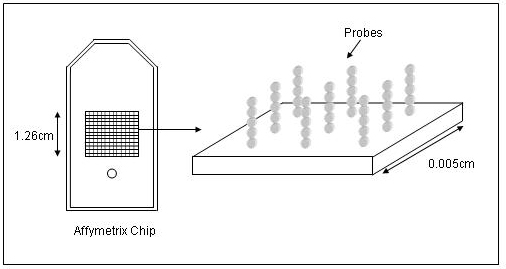
\includegraphics[width=.7\textwidth]{3microarray}
    \caption{Illustration of a typical microarray chip. Every small square can be used for an experiment to measure gene expression levels.\protect\footnotemark}
    \label{fig:3:microarray}
\end{figure}
\footnotetext{Source: http://grf.lshtm.ac.uk/microarrayoverview.htm}

Both the observational and interventional profiles are reported relatively to some average wild type profile. \citet{kemmeren2014large} report that the intervention profiles are compared to a set of 428 wild type profiles. Gene expression is measured as fluorescent intensity in the experiments. In this thesis, we work with the difference in $log_2$ fluorescent intensity between the data point and the reference wild type data, which indicates deviation from the normal gene expression levels. Because the data already indicates values relative to a norm, we choose to not preprocess the data.

% \silvan{It is unclear if the observational profiles are compared to the same set.} \silvan{ADD: measured as log2 fluorescent intensity} \silvan{ADD: some genes were excluded because they changed significantly in the WT already? see kemm. \textit{Statistical Analysis of Expression Profiles}}

There are some details of the experiments that might be of relevance in a discussion of underlying assumptions. First of all, the researchers chose to measure only a subset of about 25\% of all genes. Selection criteria included whether genes were expected to be involved in regulating other genes, and only genes were selected that do not play a vital role in keeping the cell alive (viability). 

Furthermore, the profile resulting from an experiment had to pass a quality control before being admitted to the dataset. Failing this test resulted either in repeating the experiment, or excluding the mutant. Although these checks improve the quality of the data by removing some failed experiments, they may admit some selection bias as well. 

Another form of selection bias is inherent in the experimental method. The mutant cells need to reproduce many times until a culture is grown that is large enough to do the measurements. However, cells with certain properties may reproduce quicker or easier, and be overrepresented in the measurement. It is unclear how large this effect may be.

A final factor to consider is that  data from previous work of the same institute is included in the dataset, specifically from \citet{lenstra2011specificity} and \citet{van2010functional}. The authors note that they could not find any significant differences in the data. Nevertheless, this information can be seen as a context variable, and ignoring it is an explicit modelling assumption.

\subsection{Binary Ground-Truth}
We suppose that SCMs generate the dataset. Every gene expression is interpreted as an endogenous random variable. We suppose that there is an underlying causal mechanism (function $\B{f}$) that models the relations among these gene expressions. The interventional data is generated by a SCM induced by a perfect intervention on the expression of the mutant gene, making its expression level a lot smaller. These interventions, along with the observational data, provide us with information about the SCM. 

The values in the interventional data represent deviations from the normal (wild-type) gene expressions that are measured when there is a perfect intervention on one gene (in the mutant). The more these values deviate from zero, the more likely it is that they are in fact deviating as a result of this intervention. We construct a set of binary ground-truth relations by selecting per intervened gene, those genes that respond with an absolute value exceeding some threshold. We interpret the result as a set of causes and (possibly indirect) effects. Two thresholds are used in this thesis. \citet{kemmeren2014large} used a threshold of $1.7$, stating that lower levels may be biologically relevant, but focussing on robust changes makes it more likely that they are biologically meaningful. We will also use this threshold, and introduce a lower one of $1.0$ which allows us to use more information of the system, and evaluate against a larger (but noisier) set of ground-truth values. 
% \silvan{Risk: high variance genes (why?), option: filter; why no other preprocessing? log2 diff is already something}

Often, we restrict ourselves to the 1.484 intervention genes (i.e. genes that occur in the intervention data as object of a perfect intervention) as possible effects, instead of all 6.182 measured genes. This makes it easier to interpret our metrics, because every relation between these genes is captured by the interventional data. We call this subset of the intervention data the \textit{intervention table} $\B{X} \in \mathbb{R}^{1479\times 1479}$ where $\B{X}_{ij}$ is the relative expression level of gene $i$ in the experiment with gene $j$ knocked out (i.e. intervened upon). When subjected to some ground-truth threshold, we get a matrix of the same dimensions that is true where gene $j$ is a cause of gene $i$.

We use the binary ground-truth to analyse the dataset, to inform our algorithm to find an order in the genes, and to evaluate causal methods. Scientific knowledge about some relations could be used to evaluate our methods as well, but it is incomplete and somewhat obscure because it is scattered about many papers with different experimental methods and conditions. 

\subsection{Properties}

Certain properties of the dataset are valuable to interpret our inference challenge, and justify the assumptions of our methods. The most challenging property of the dataset is \textbf{sparsity}. The data can be interpreted as a collection of single samples from (slightly) different joint distributions, since there is only one measurement of the genes per intervention. The exception is the observational data, which consists of 262 samples of the same distribution.

\begin{figure}[h]
    \centering
    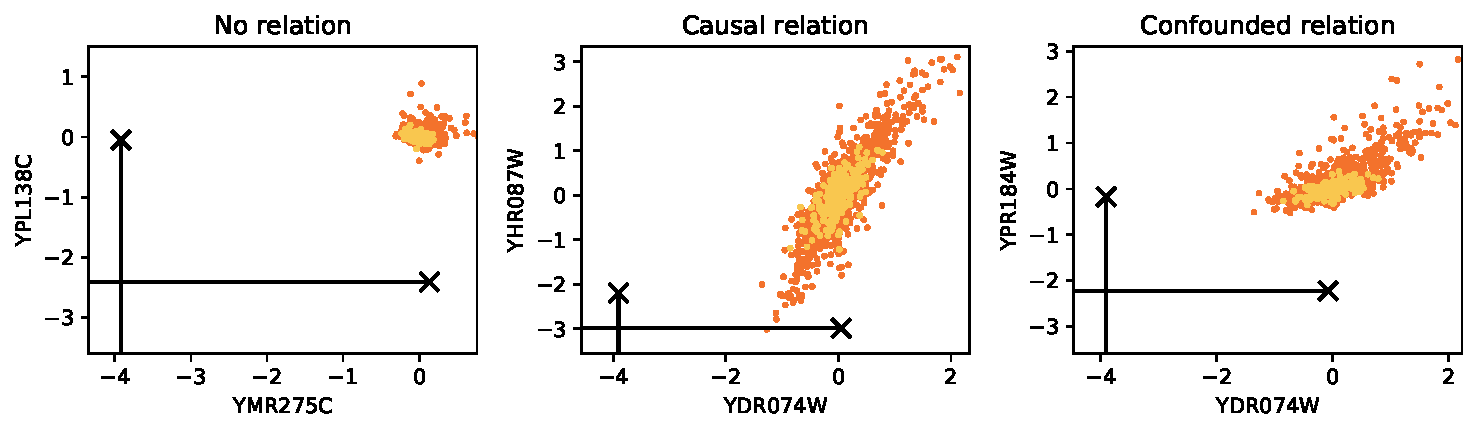
\includegraphics[width=\textwidth]{3gene_vs_gene}
    \caption{Expression levels of pairs of genes. All observation values are shown in orange, all intervention values in blue. The black crosses show the interventions on the plotted genes, the line shows which gene was intervened on.}
    \label{fig:3:genevsgene}
\end{figure}

\begin{figure}[h]
    \centering
    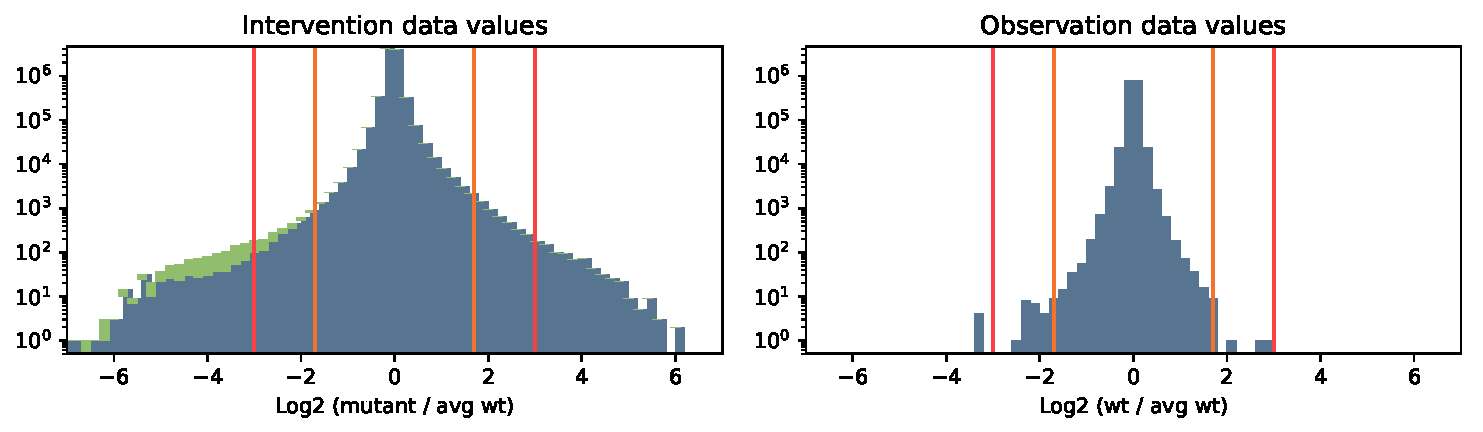
\includegraphics[width=\textwidth]{3data_values}
    \caption{Distribution of expression values in observation and intervention data. The values of the mutant genes themselves are shown in green. The ground-truth thresholds are shown in the intervention plot.}
    \label{fig:3:datavalues}
\end{figure}

\begin{figure}[h]
    \centering
    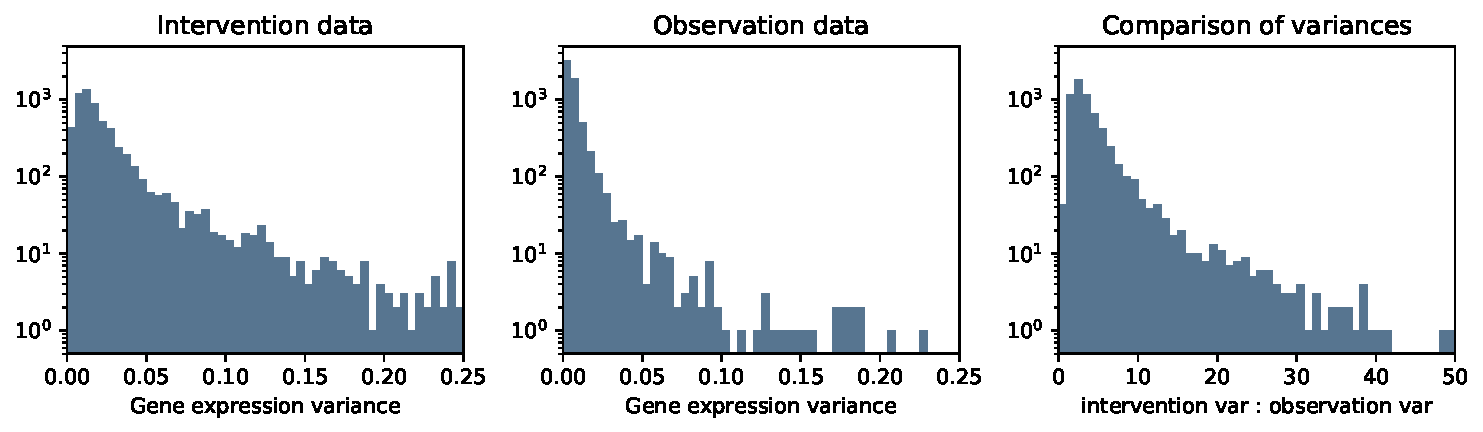
\includegraphics[width=\textwidth]{3gene_variance}
    \caption{Distribution of variance in the expression values of single genes in the observation and intervention data. The distribution of the ratio between intervention variance and observation variance per gene is shown on the right.}
    \label{fig:3:datavariance}
\end{figure}

Figure \ref{fig:3:genevsgene} shows examples of possible relations between two genes, distinguishing observation and intervention data. The relation between two variables can be visually estimated in these plots. In the middle plot, we see that the genes are correlated. By Reichenbach's principle we infer that there is some causal relation. Gene \textit{YHR087W} has reduced expression when we intervene on gene \textit{YDR074W}, but not the other way around. We may conclude that gene \textit{YDR074W} is an ancestor of gene \textit{YHR087W}. In the right plot we see two genes that are correlated, but do not respond to interventions. This indicates confounding.

Generally, the intervention data has higher \textbf{variance}, because the effect of the intervention propagates to many genes. Figure \ref{fig:3:datavalues} shows that the interventional data contains more extreme values. Figure \ref{fig:3:datavariance} compares the variance of genes in the observational and interventional data. In the interventional setting, the variance of genes tends to be about three, in some cases even more than ten times larger.

\begin{figure}[h]
    \centering
    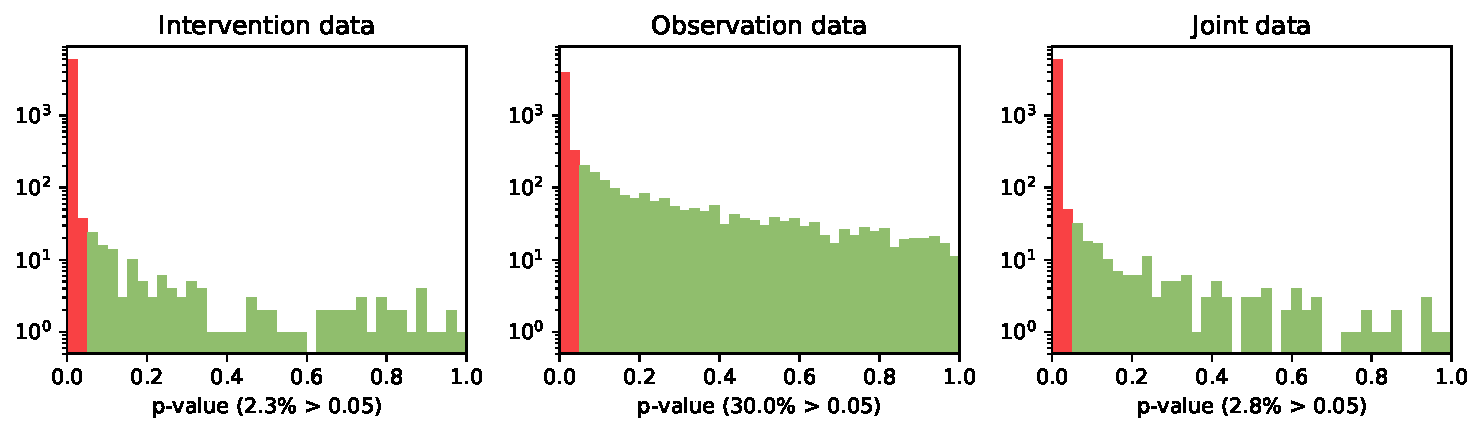
\includegraphics[width=\textwidth]{3normality}
    \caption{Distribution of p-values from the Shapiro-Wilk normality test per gene. For the intervention and joint data, we sampled 262 values per gene to make the p-values comparable.}
    \label{fig:3:normality}
\end{figure}   

The partial correlation test is commonly used in the causality literature to test if two variables are dependent or independent\footnote{When the test fails to reject the hypothesis of dependence, it is commonly concluded that the variables are dependent.} This test relies on the assumption that the data is \textbf{normally distributed}. Figure \ref{fig:3:normality} shows the results of a Shapiro-Wilk normality test. The normality assumption is more valid for the observational data than for the interventional data. This is to be expected, since we model the observational data to be sampled from a single distribution with some noise, and the interventional data from different distributions. Based on this test, visual inspection of the data as in Figure \ref{fig:3:genevsgene} and the general distribution of values in \ref{fig:3:datavariance}, we conclude that the normality assumption is acceptable. Nevertheless, different independence tests can still be interesting since they can capture other forms of independence. 

\begin{figure}[h]
    \centering
    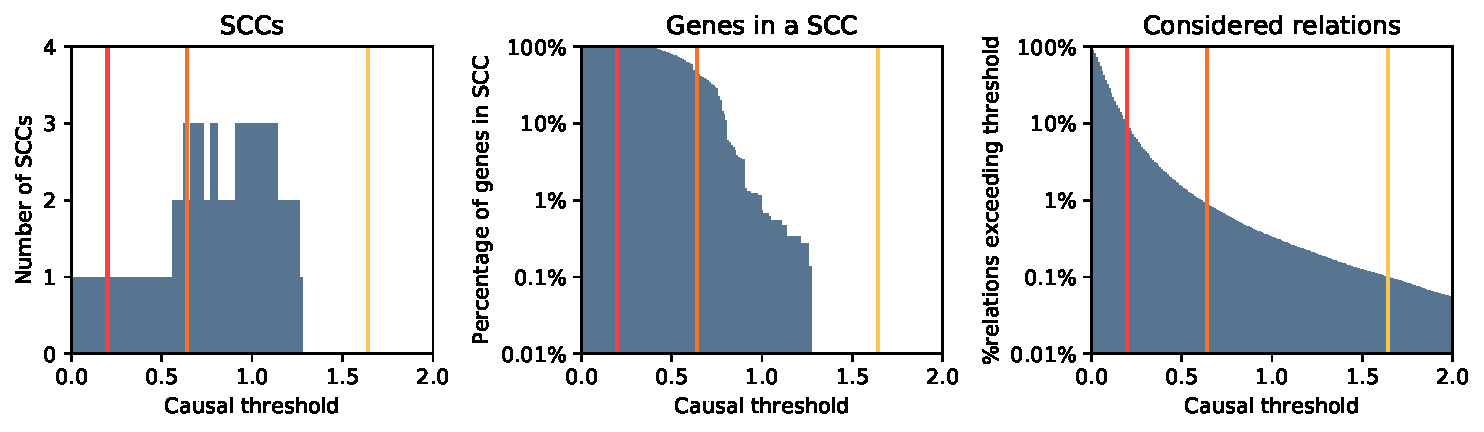
\includegraphics[width=\textwidth]{3cycles}
    \caption{Left: number of SCCs in the graph per ground-truth threshold. Middle: percentage of intervention genes that are in a SCC per threshold. Right: percentage of causal relations that are significant according to the threshold.}
    \label{fig:3:cycles}
\end{figure}    

Some causal inference methods, including our order-based LCD, assume that there are no \textbf{cycles} in the underlying graph. We construct a graph from the binary ground-truth and compute the number of strongly-connected components (SCCs): the number of variable subsets in which there is a directed path from each variable to each other variable. Combined with the number of variables in SCCs, this gives an indication of the validity of the acyclicity assumption. The results in Figure \ref{fig:3:cycles} show that for any ground-truth threshold, the number of SCCs is small. At the $1.7$ threshold, there are no SCCs and therefore no cycles. At the $1.0$ threshold, there are SCCs and only about $1\%$ of variables are in them. We conclude that acyclicity is an acceptable assumption, and it is a valid approach to search for a causal order of genes as a first step in our algorithm.

\begin{figure}[h]
    \centering
    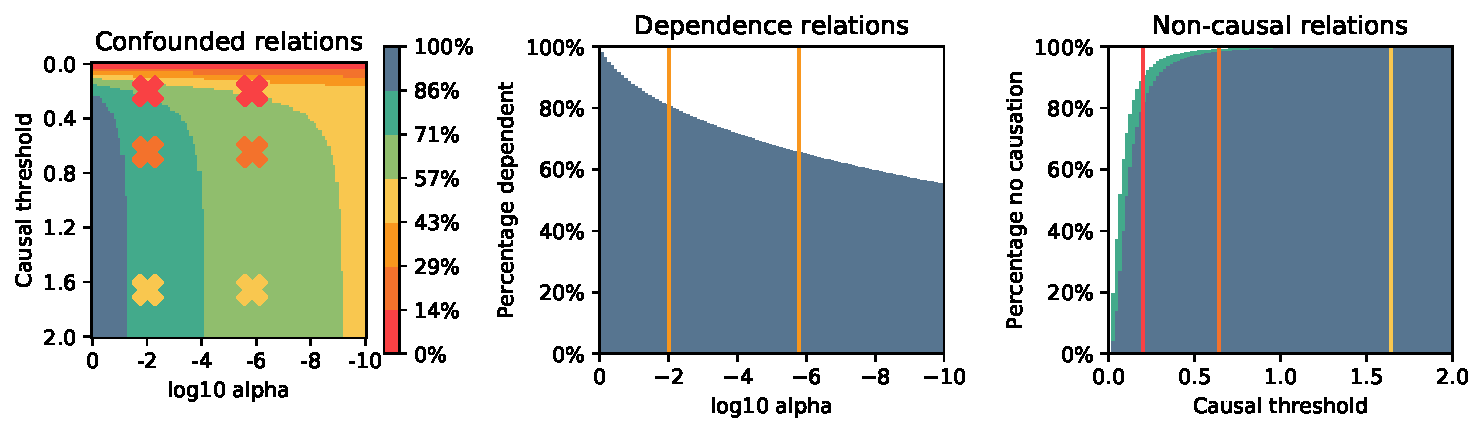
\includegraphics[width=\textwidth]{3confounding}
    \caption{Left: percentage of relations that are only related by confounding, for different binary thresholds, and significance levels. The two crosses show the alpha and thresholds used in this thesis. Middle: percentage of relations that are dependent per significance level. Right: percentage of relations that are not causal per binary ground-truth threshold (inverse of Figure \ref{fig:3:cycles}-right)}. Lighter color represents the knock-out values.
    \label{fig:3:confounding}
\end{figure}    

Next we test the frequency of \textbf{confounding} in the data. We could search for common ancestors in the binary ground-truth, but this will not find latent confounding. Therefore, we test for each variable pair if they are dependent (by the partial independence test), and not a cause of each other in the ground-truth. Note that we will miss variable pairs in which one variable causes another, while also being confounded. Figure \ref{fig:3:confounding} shows that at our ground-truth thresholds, and a significance level of $\alpha = \frac{1}{N} \approx 0.00057$, about $80\%$ of all relations among intervention genes is confounded. Note that both ground-truth thresholds are quite strict, so we mainly measure dependence among genes. We suspect that in the gene expressions are highly interconnected, explaining dependence between most genes. However, most of the relations are indirect and have relatively small effect, which makes it hard to infer the causal structure. Large prevalence of latent confounding is acceptable, since most methods can deal with it. However, the recall of LCD may be quite limited. It cannot identify ancestral relations that are also confounded, meaning that an expected $80\%$ of all relations are already disqualified.


\subsection{Relevance, tasks and state-of-the-art}

Due to the sparsity of the data, any kind of causal inference task is challenging. The few methods that have been applied on this data improve over some baseline only in a small number of strongest predictions. ICP is the method with the best performance. LCD has been tested as much faster alternative. Preselection is commonly used to speed up the algorithms, and might even improve accuracy of the most certain predictions. Three papers are shortly discussed in this subsection.

The ICP algorithm was first proposed by \textbf{\citet{peters2016causal}}, and tested on multiple datasets including the one of \citet{kemmeren2014large}. Two versions of ICP are designed, one with a test on regression coefficients, the other as faster alternative with an approximate test of residuals. L2-boosting regression \citep{schapire1998boosting} is used to preselect variables. Effects are considered true if the absolute intervention value exceeds the upper or lower $1\%$ of the observation values per gene, resulting in about $9.2\%$ of all effects being true. 6 out of the top 8 predictions of both ICP versions are true. A baseline that uses correlation on the pooled data has 2 true predictions in the top 8.

\textbf{\citet{meinshausen2016methods}} use ICP in a slightly different way, and evaluate against a different definition of true effects. They introduce a generalized ICP that accounts for latent confounding. They use stability selection \citep{meinshausen2010stability} to make a larger number of more fine-grained predictions, visualised in a receiver operating characteristic (ROC) curve. Effects are considered true only if the values of the cause and effect gene are extremes in the joint data, leading to a strict ground-truth set of about $0.1\%$ of all effects. The normal ICP version predicts 7 true effects in the first 9 predictions, and makes not one other true prediction in the top 25. The generalized ICP version predicts 5 true effects in the first 8 predictions and keeps making true predictions at a declining rate after that. A baseline using cross-validated sparse Lasso regression is provided for comparison, but it performs worse than random.

The most recent work on causal inference applied to the \citet{kemmeren2014large} dataset is by \textbf{\citet{versteeg2019boosting}}, who combine elements of both papers and investigate LCD as an alternative method that is faster. Predictions are made using stability selection. L2-boosting regression preselection is used for ICP and as an option for LCD. Two independence tests are compared, but no significant difference in performance is found. True effects are defined by the top $x\%$ absolute value in the intervention data. Methods are compared on a ROC curve, at ground-truth thresholds $10\%$, $1\%$, and $0.1\%$, but the comparative results are the same. In the first 100 predictions, ICP performs best, followed by LCD using preselection. An interesting result is that a baseline using only the preselection method outperforms the methods thereafter. LCD without preselection performs worse than this baseline from the start. ICP predicts about 40, 20, and 10 effects correctly in the first 100 for the respective ground-truth thresholds.

% \citet{tibshirani1996regression} Lasso regression


% 5 pages

\newpage
\section{Approximating Variable Order}
\label{chapter:methodorder}

% 7 pages

% SECTIONS
% Distinction order and inference problem
% Model options and justification of decision
% Algorithm description (2)
% Derivations for Expectation Propagation (1)
% Assumptions and justification
% Short validation on synthetic data
% Short comparison to baselines


% NOTES
% Uhler shows that order is useful

% Results:order -> Method I (order)
% Distinction order / inference
% Modeling decisions, justification of metrics
% Description of methods/baselines
% Evaluation
% Decision
% Afronding


% Intro: order VS inference problem (Uhler?), modeling options and decision (ignore observation genes)
% Methods:
% - Metric: penalty, random baseline
% - Edmond: minimum weight directed spanning tree
% - Evolution Strategy continuous: directly optimize
% - ES discrete
% - Scoring(?): TS, SA, PR
% - Sun
% Results / Comparing methods:
% - Penalty VS N
% - Score over order
% - sorted TS: sorted data


\subsection{Methods}


The genes in the dataset can be ordered according to their position in the ancestral hierarchy. This order is clearly defined when there are no cycles in the underlying graph. When cycles do exist, we can only infer some order that satisfies many ancestral relations. We hypothesize that an approximation to this underlying topological order can be leveraged to improve causal discovery.

If we ignore the purely observed genes that do not occur as knock-out gene, we are left with a square \textit{intervention table} $\B{X} \in \mathbb{R}^{N\times N}$. $X_{ij}$ is the relative expression level of gene $i$ in the experiment with gene $j$ knocked out. If we take into account all intervention data, we have $N=1479$ genes. This table represents a complete directed graph if it is interpreted as a weighted adjacency matrix. A straightforward way to model the problem of finding order, is to minimize the sum of the absolute weight of the edges that violate the order $\pi$, which is represented by a permutation of genes. We call the average absolute weight of violating edges the \textit{penalty} $p_\pi$:

$$p(\pi) = \frac{\sum_{\pi_i < \pi_j}|X_{ij}|}{\frac{1}{2}N(N-1)}$$

$N$ is the number of intervention genes. To make this number more interpretable for different intervention tables, we define the \textit{penalty ratio} $r_\pi$ as the penalty divided by the average absolute value of all relations, excluding values of the knocked-out genes themselves. We present this value as a percentage. A random order is expected to have a penalty ratio of $100\%$.

$$r(\pi) = \frac{\sum_{\pi_i < \pi_j}|X_{ij}|}{\frac{1}{2}N(N-1)} \frac{N(N-1)}{\sum_{i \neq j}|X_{ij}|} = \frac{2 \sum_{\pi_i < \pi_j}|X_{ij}|}{\sum_{i \neq j}|X_{ij}|}$$

Assuming that the expression values reflect the importance of ancestral relations, we can weigh the edges by the respective expression values. In an unweighted variant, we could add only those edges whose expression value exceeds some threshold. This yields a sparser graph that may still contain cycles. It is important to realise that this thresholding has different meaning and implications than the thresholding on which we may base our evaluation of predictions. In testing predictions, we are interested in meaningful relations. In finding order, we are more pragmatic and could use any threshold that yields the best prediction algorithm.

\subsubsection{Minimum Feedback Arc Set Problem}
The presence of cycles in the underlying graph is an important challenge to inferring order. Finding the order in an acyclic graph is trivial and can be computed with a complexity linear in the number of nodes and edges (for example Kahn's algorithm \citep{kahn1962topological}). One way to find a good ordering in graphs with cycles, is to eliminate edges to make the graph acyclic, without too much damage to the hierarchy. An order is then found in the acyclic subgraph.

This strategy can be modeled as the Minimum Feedback Arc Set (MFAS) problem. The minimum feedback arc set is the smallest set of edges whose elimination makes the graph acyclic. A weighted version of the problem aims to find the set of edges with minimal summed weight whose elimination makes the graph acyclic.

In theory, we could find the optimal solution for the complete directed graph constructed from the intervention table, eliminate the minimal feedback arc set, and use Kahn's algorithm to infer an order in the remaining acyclic subgraph. Unfortunately, the MFAS problem is expensive to solve. In fact, \citet{guruswami2008beating} show that even approximating the maximum acyclic subgraph problem with an approximation ratio lower than $0.5$ is Unique-Games hard. That is, it is impossible to get a polynomial-time approximation of the minimal feedback arc set that is better than imposing a random order.

Because of the complexity of the problem, we focus on heuristic methods to eliminate edges, or optimize the order directly with respect to the penalty. We first discuss approaches that use the continuous values of the intervention table, followed by approaches that first binarize the data with some threshold. Finally, we discuss our experiment and results, justifying the algorithms that we use in the causal inference method described in the next chapter.

\subsubsection{Continuous approaches}

A straitforward approach is to directly optimize the penalty. Because it is expensive to find the optimal solution, we designed an \textbf{evolution strategy} (ES) to search for a good solution\footnote{cf. \citet{eiben2003introduction} for an introduction to evolutionary algorithms.}. This method iteratively updates a \textit{population} of solutions according to evolutionary principles. A solution in this case is a permutation of variables, which are initialized randomly. Every iteration, we \textit{recombine} pairs of solutions to form new solutions\footnote{Usually, recombination is followed by mutation - small random changes to the solution. We found no mutation method with a strong effect on the penalty and decided to leave it out.}. The penalty of each new solution is computed and the best solutions are kept in the population. We experimented with different recombination methods and different parameters on synthetic data and selected a good setting for the experiments in this chapter. 

The population consists of 100 solutions. We use cycle crossover \citep{oliver1987study} as recombination method, which preserves the absolute position of indices in the permutations. If we have two permutations $\pi^1$ and $\pi^2$, we first identify all \textit{cycles} $C_k \subseteq \{1...N \}$ such that $\{\pi^1_i \} = \{\pi^2_i \}, i\in C_k$. The indices in a cycle can be swapped between the two permutations. The new solutions are formed by swapping alternating cycles: $\pi^1_i \ot \pi^2_i, \pi^2_i \ot \pi^1_i \text{ for all } i\in C_k, k \text{ even}$.

Another approach is inspired by implicit assumption that the underlying graph is acyclic. We interpret the intervention data as a noisy weighted adjacency matrix of this graph, and wish to find an order in accordance with the largest values in the matrix. To find this order, we first use the \textbf{Edmonds algorithm} \citep{edmonds1967optimum} to find the spanning arborescence of maximal weight, i.e. a rooted directed tree spanning all nodes such that the values on the selected edges are maximal. For these values we take the absolute intervention values. When we have this arborescence, we can select an order of nodes that satisfies it, for example using Kahn's topological sort algorithm \citep{kahn1962topological}. 

The Edmonds algorithm has complexity $O(EV)$. When we use the complete intervention table, this scales with the number of genes to the power 3. We propose a faster \textbf{Sparse Edmonds algorithm} that scales with power 2, by allowing only a maximum number of edges to be added per node. In our experiment we use the top $10$ edges with highest absolute value.

\subsubsection{Discrete approaches}
% Context: what was it designed for?
% Algorithm: how does is work?
% Extensions: how to include continuous values?

We also investigate some approaches using binarized intervention data. Subjecting the data to a threshold makes it possible to use some methods, at the cost of information loss. First, we applied a very similar \textbf{evolution strategy} to the binary data. Solutions are now selected based on a \textit{binary penalty} computed from the binarized data. Because the ES is designed to directly optimize some objective, we see that obfuscating this objective is detrimental to its performance.

A different approach to approximating order is to rank the nodes in a graph. We interpret the binarized intervention data as an adjacency matrix of an unweighted directed graph. Three methods were applied to assign a score to the nodes of the graph, and we infer an order by sorting the nodes by their score and randomly deciding ties. These methods were all designed with a specific application in mind, which means there is no a priori guarantee they will work well on our problem.

Furthermore, the methods are not symmetrical. We can construct a graph with edges from cause to effect and determine the order by sorting one way, or construct the graph with edges from effect to cause and sort reversely. Both approaches will yield a different result. 

\textbf{PageRank} \citep{page1999pagerank} was developed to score the relative importance of web pages, based on hyperlinks. The score represents the probability that a fully randomized user clicking hyperlinks, ends up on some website. The scores can thus be interpreted as a probability mass function over nodes. The score of one node in the graph depends on the score of the parent nodes linking to it, and to how many other nodes the parents link. This last factor is undesirable in our context. If some node has edges to multiple other nodes that have no other edges, they will likely have a lower score than their parent (see for example Figure \ref{fig:4:scores}). 

PageRank can be adapted to allow weighted edges. For example, \citet{tyagi2012weighted} use the frequency of clicks per link to determine the probability of moving to another page, instead of a uniform probability over all links.

Where the PageRank score is intended as probability of reaching a website $X$ by random clicking, we loosely interpret it as either the likelihood that a random intervention affects gene $X$, or reversely that a random effect was caused by an intervention on gene $X$. A high PageRank score should correspond to a low resp. high position in the causal order\footnote{Genes that are high in the causal order are expected to be causes of lower genes.}.

\textbf{Social Agony} was proposed by \citet{gupte2011finding} to analyse hierarchy in social networks. Users of a directed social medium are assigned a discrete score that is computed based on who follows who. Formally, the group of users is subdivided as a partially ordered set, because we cannot distinguish between users with the same score. The granularity in our experiments will prove to be so low that it hurts the performance. 

The algorithm assigns a rank to every user. Users are said to experience agony when they follow someone of lower rank. This agony is usually computed as the difference of their rank plus one. The algorithm then assigns ranks to users such that the total agony of all users is minimized. A version of Social Agony with weighted edges was proposed by \citet{tatti2015hierarchies}, in which the agony of each follow-relation is weighted by the corresponding edge weight. We did not test this version here.

In the original formulation, agony is caused by following users of lower rank. We see it as a penalty for a gene that has an effect on a potential cause, i.e. a gene higher in the order. The score then corresponds to an order in which genes minimally affect these potential causes. In the reversed case, agony is a penalty for being affected by a potential effect gene lower in the order, with a score corresponding to an order in which genes are minimally caused by their potential effects.

The final scoring algorithm is \textbf{TrueSkill}, proposed by \citet{herbrich2007trueskill}. It is used to assign a skill level to players of an online video game, based on match outcomes. The set of all matches is modeled with a factor graph. The skill of a player $s_i$ is normally distributed with some mean $\mu_i$ and variance $\sigma_i^2$. The player's actual performance $p_i$ is also normally distributed with his skill as mean, and some constant variance. The match outcome is determined by the difference of the performances $d_{ij}$. The sum-product algorithm \citep{kschischang2001factor} is used to compute the parameters of each player's skill distribution. The expectation propagation algorithm \citep{minka2001family} is used to approximate a distribution of each performance difference $d_{ij}$ as a normal distribution. In ranking the players of a game, it is important that a high rank cannot be achieved with a lucky win against a highly ranked player. Therefore, the TrueSkill score penalizes uncertainty and is defined as $\mu_i - 3\sigma_i$. 

Applied to the gene perturbation data, we interpret a high score as an indication that some gene is a very likely cause of some other genes with high certainty. It should be high in the causal order. In the reverse case, a high score indicates a gene that is very likely an effect of some other genes with high certainty, and should be low in the causal order. No simple adaptation of the algorithm was found with weighted matches, which we could use to include the intervention values. 

The last method to be discussed is an algorithm developed by \citet{sun2017breaking}, we will call it \textbf{Sun's algorithm}. In the context of crowd-sourced taxonomy graphs, it's aim is to break cycles (which are logically inconsistent in a taxonomy), while preserving the logical structure. This problem is very close to the MFAS problem, which is too expensive to solve exactly. Once the graph is acyclic, it is trivial to infer some variable order.

The algorithm consists of two steps. First, the nodes in the graph are scored. Then, strongly connected components (SCCs) are iteratively broken by removing edges based on the node scores. \citet{sun2017breaking} compare TrueSkill and Social Agony scoring, and propose three heuristic strategies to break cycles. The \textit{greedy strategy} selects the edge that violates the hierarchy the most, i.e. with the largest difference between node scores. The \textit{forward strategy} selects all outward edges of the node highest in the hierarchy. The \textit{backward strategy} selects all inward edges of the node lowest in the hierarchy. Next to the six configurations that can be made, they provide an ensemble voting method. For each edge we count by how many configurations it is removed. Edges are iteratively removed in order of the number of votes, until there are no more cycles. 

Because this method is much more time-consuming then the other ones, we selected two based on a small experiment. The voting method was selected, because it most often removes the smallest number of edges, indicating that it comes closest to approximating a solution to the MFAS problem. The greedy strategy combined with TrueSkill scoring was chosen because it  generally performs best out of the individual methods. As mentioned earlier, the superior performance of the TrueSkill scoring is most likely due to the information loss in the discrete scores of Social Agony. We only applied these two methods to a graph with edges from effects to causes. This seems more natural in analogy with the taxonomy application. 


\subsection{Experimental Results}

We compare the algorithms based on the penalty ratio, and computation time. We test each algorithm on samples of the data, varying the sample size $N$ from $2$ to $1.479$, the full dataset. Every algorithm is tested on the same 5 random samples for each sample size. Some algorithms become very time-consuming to evaluate, and were not tested on larger samples. Note that the variance in penalty and time results from two factors, variance in the sample (especially for small samples) and variance in the algorithm due to randomness. 

\subsubsection{Global Results}

\begin{figure}[h]
    \centering
    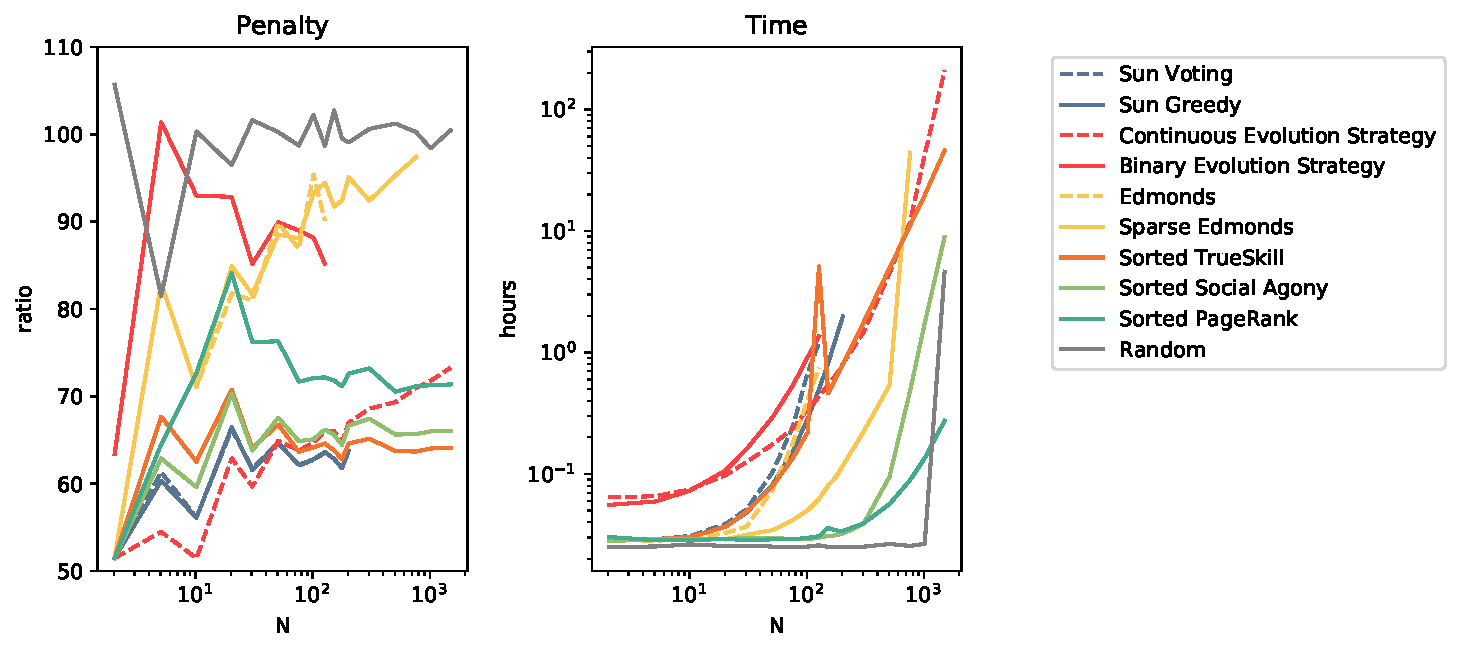
\includegraphics[width=\textwidth]{4algorithm_global_comparison}
    \caption{Comparison of penalty ratio and computation time. Averages of results over 5 data samples are shown. Variance generally decreases when sample size increases. It is left out of the graphs to keep them readible.}
    \label{fig:4:general}
\end{figure}  

The comparison of penalty ratio and computation time between all algorithms is shown in Figure \ref{fig:4:general}. At smaller sample sizes, the continuous evolution strategy performs best. This is the only algorithm that attempts to directly optimize the penalty ratio. Because this optimization problem is easy for small samples, this result is to be expected. For larger samples its performance decreases, and the computation tim becomes much longer. 

When the samples get larger, the score ordering algorithms and the two versions of Sun's algorithm outperform the others. Of the score ordering algorithms, TrueSkill performs best, followed by Social Agony and PageRank. The order of computation time is reversed, PageRank being the fastest followed by Social Agony and TrueSkill. The two versions of Sun's algorithm seem just a little better than ordered TrueSkill, at the expense of a much longer computation time. Because of this, we select TrueSkill as the most useful algorithm for our causal inference method.

\subsubsection{Score Ordering Algorithms}

The score ordering algorithms perform well and are relatively fast. Therefore, we look at them in some more detail. These algorithms can be applied in two ways. In the \textit{forward} interpretation, we construct a graph with edges from effect to cause (observed to intervention variable). Variables with a higher score are higher in the causal order. In the TrueSkill model for example, causes are winning from effects and get a higher skill level score. In the \textit{backward} interpretation, edges point from cause to effect. Variables with a higher score are lower in the causal order. Because the algorithms are not symmetrical, these two interpretations do not yield the same results. The same interpretations can be applied for the Edmonds algorithm, in constructing the (sparse) weighted graph in which the minimal branching is found.

\begin{figure}[h]
    \centering
    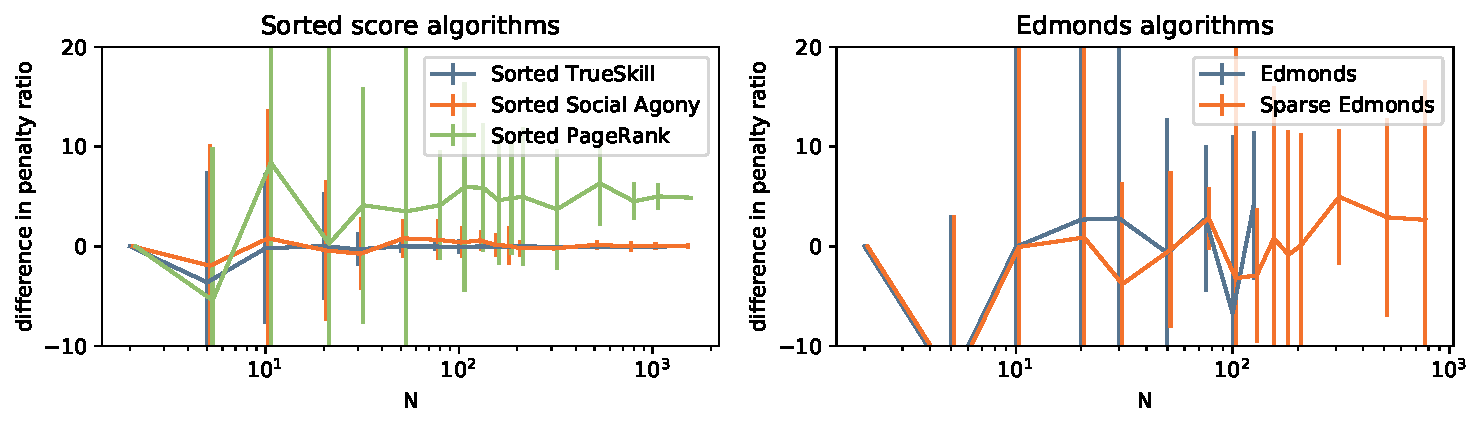
\includegraphics[width=\textwidth]{4difference_forward_backward}
    \caption{Average difference between Forward and Backward algorithms over 5 samples per sample size. Vertical bars show two standard deviations. A positive difference means that the Backward algorithm has lower penalty.}
    \label{fig:4:forwardbackward}
\end{figure}  

Figure \ref{fig:4:forwardbackward} shows the difference in the penalty ratio between the forward and backward interpretations. For the larger sample sizes, we see that especially PageRank and Sparse Edmonds perform better with the \textit{backward} interpretation (positive difference). TrueSkill, Social Agony and Edmonds show only small differences. In this thesis, whenever the interpretation is not mentioned, we used the \textit{backward} version of these algorithms. 

\begin{figure}[h]
    \centering
    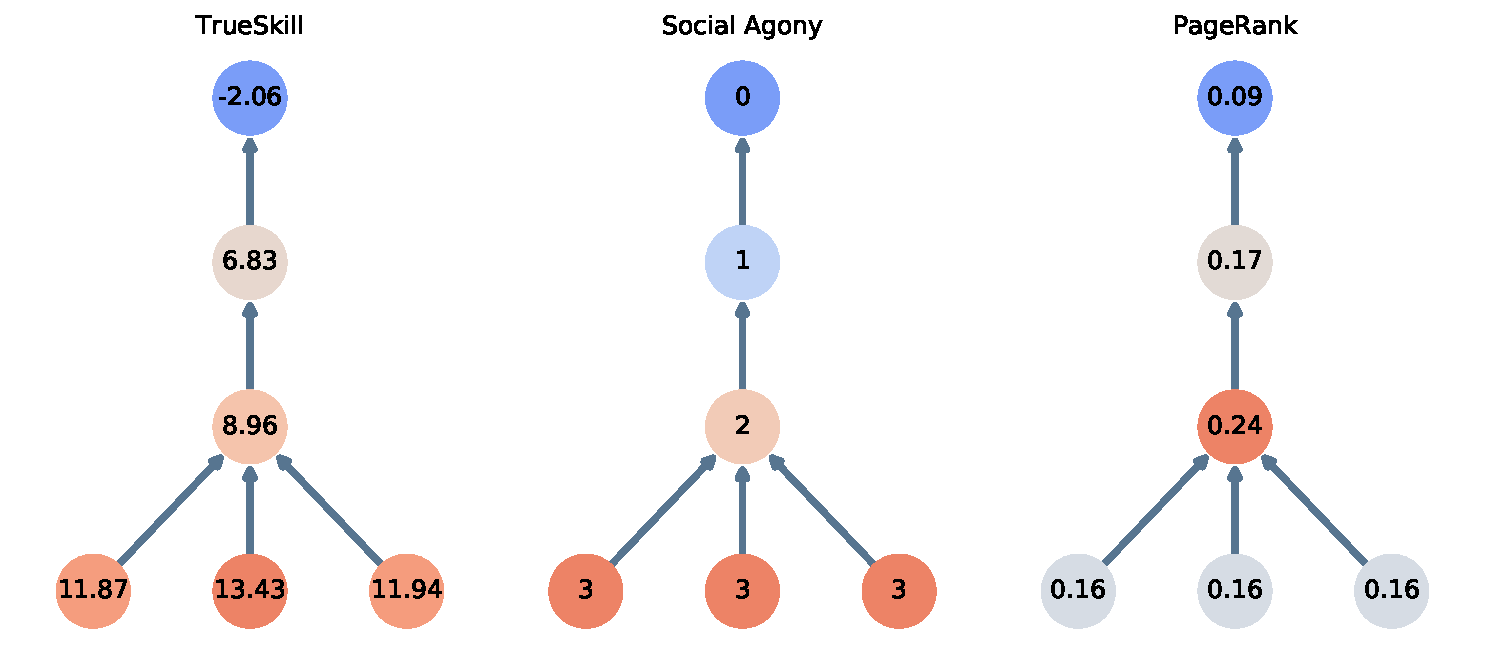
\includegraphics[width=\textwidth]{4score_examples}
    \caption{Example scores of backward score sorting algorithms.}
    \label{fig:4:scores}
\end{figure}  

Figure \ref{fig:4:scores} shows per algorithm the score it assigns to nodes in a simple graph. The edges point from effect to cause, and are thus reversed for the algorithms. It can be seen that the continuous scores of TrueSkill are somewhat arbitrary. Social Agony is easier to interpret. This specific graph also highlights a weakness of PageRank. The three bottom nodes share the score of their cause, which results in a lower relative score.

\begin{figure}[h]
    \centering
    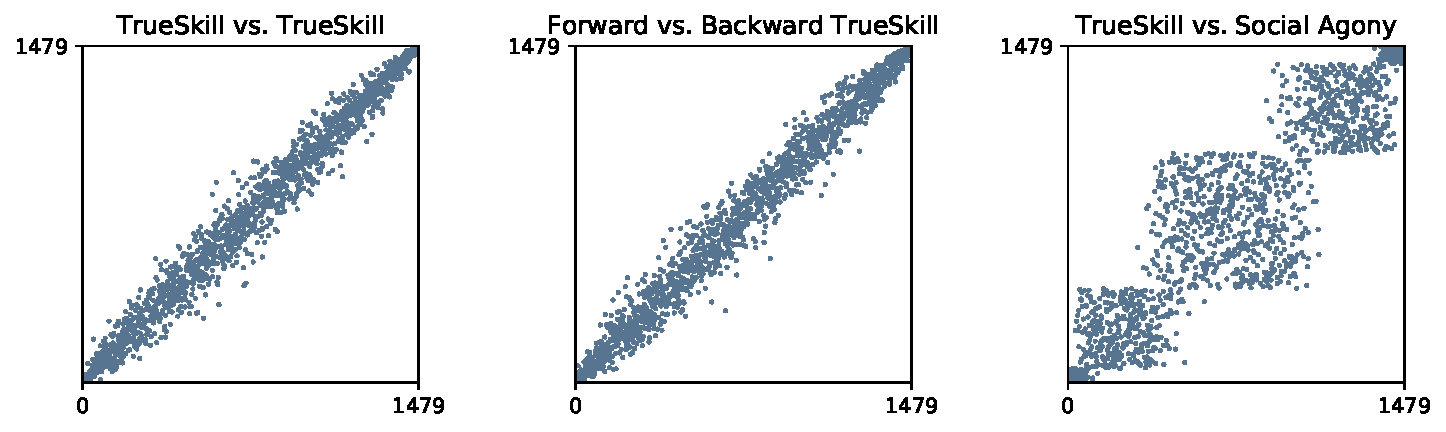
\includegraphics[width=\textwidth]{4order_consistency}
    \caption{Consistency between order algorithms.}
    \label{fig:4:consistency}
\end{figure}  

\begin{figure}[h]
    \centering
    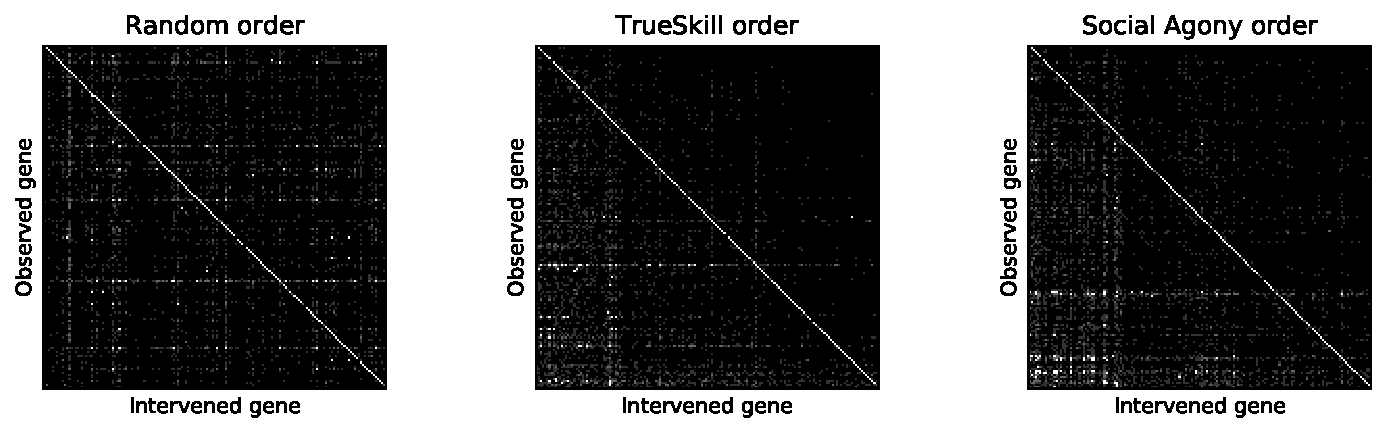
\includegraphics[width=\textwidth]{4ordered_data}
    \caption{Ordered intervention tables.}
    \label{fig:4:ordered}
\end{figure}  

A comparison between the infered orders is shown in Figures \ref{fig:4:consistency} and \ref{fig:4:ordered}. Figure \ref{fig:4:consistency} compares the one instance of the order found by the TrueSkill algorithm to three other orders. It shows per gene, at what index that gene is placed by the other order. On the left we compare two orders infered using TrueSkill. The variance is only due to randomness in the algorithm. TrueSkill quite consistently puts genes in about the same position in the order. The variance seems to be somewhat lower at the extremes, indicating more certainty about the most obvious causes and effects. In the middle we compare the forward and backward versions of TrueSkill. The figure is very similar, corresponding with the small difference in penalty ratio that we found earlier. On the right we compare TrueSkill with Social Agony. We see that the Social Agony algorithm distinguishes between five discrete scores. The order of genes with the same score is decided randomly. Again, there is more certainty about the extremes of the order. Interestingly, these two algorithms infer a very similar order, Social Agony just has a lower granularity in its scoring. Although this allows TrueSkill to achieve a somewhat better penalty ratio, the Social Agony score may be more informative and useful for causal inference. 

A further comparison between these two algorithms is shown in Figure \ref{fig:4:ordered}. The intervention table is shown with the absolute values grouped into four ranges with corresponding shades of gray. Genes are ordered in the same way on the x-axis and y-axis. High values have the brightest color. On the diagonal we see a bright line, indicating the expression levels of the genes that are interevened upon. The top-right triangle shows all relations that are violated by the order, and should thus be as dark as possible. Comparing TrueSkill (middle) and Social Agony (right), we see that Social Agony pushes the extreme values as far from the diagonal as possible. These genes fall into the two groups with the highest rank. TrueSkill can make a more detailed distinction between genes. Being able to spread out the most extreme values more, it achieves a better penalty ratio.  

% 6 pages

\newpage
\section{Causal Discovery using Order-Informed Context}
\label{chapter:methodcontext}

% SECTIONS
% LCD/ICP
% Design of context variables and justification of decisions
% Assumptions and justification
% Short validation of synthetic data

\subsection{Local Causal Discovery}

% intro
Local Causal Discovery (LCD) was originally proposed by \citet{cooper1997simple} as a fast, incomplete algorithm. It can determine a direct causal relationship between two variables in a system of three variables. It can also be applied to a larger system by marginalizing over variable triples and testing for ancestral relationships between variables. 

% motivation
LCD is chosen as the causal inference method in this thesis because it is simple, and a good trade-off between performance and computation time. It was applied to the \citet{kemmeren2014large} dataset by \citet{versteeg2019boosting}. They compared LCD to ICP \citep{peters2016causal}, presenting a somewhat higher precision in the top predictions with ICP, at the cost of three times the computation time. 

\subsubsection{Assumptions}

The algorithm tests a causal relation $X\to Y$ between two endogenous variables, using a third exogenous variable $C$ (the context). A small set of statistical independence tests restricts the set of possible causal subgraphs with nodes $X$, $Y$ and $C$. Under some circumstances, it allowes us to infer  that $X$ is an ancestor of $Y$.

LCD relies on some assumptions. Like many inference algorithms, the starting point is to model the underlying system as a SCM. The context variable needs to be exogenous, such that no system variable can be its cause. Causal faithfulness is assumed to link (in)dependences to the d-separation of variables. To measure these (in)dependences from the data, the dependence and independence tests are taken as oracles, such that their outcomes are taken as the truth. Unbiased data selection and acyclicity are also assumed. The acyclicity could be relaxed, as in a more recent formulation of LCD by \citet{mooij2016joint}. However, the development of the LCD method is not the focus of this thesis.

\subsubsection{Statistical tests}

LCD discovers those causal relations, which effect can be measured from the data as $\Prb _M(Y|do(X=x)) = \Prb _M(Y|X=x)$. This is the case when there is no confounding between $X$ and $Y$, no effect of $Y$ on $X$, and no effect of $C$ on $Y$ that bypasses $X$. Figure \ref{fig:5:lcdgraphs} shows the three subgraphs that satisfy the condition. Note that all possible relations between $C$ and $X$ given the exogeneity assumption are allowed.

\begin{figure}[h]
    \centering
    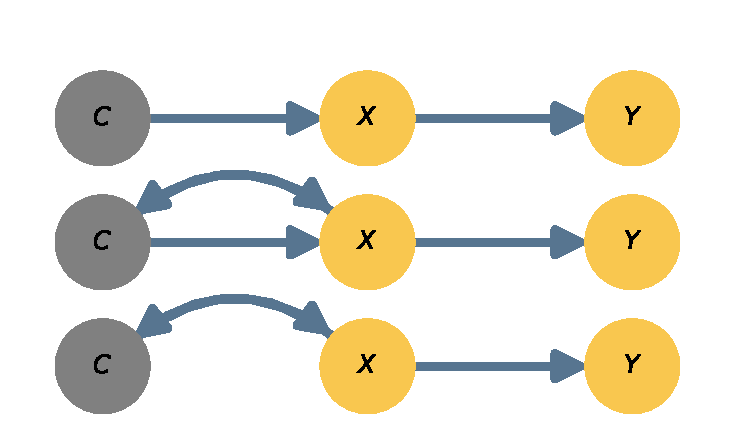
\includegraphics[width=.6\textwidth]{5LCDgraphs.pdf}
    \caption{All mixed graphs in which LCD can infer the relation $X\to Y$}
    \label{fig:5:lcdgraphs}
\end{figure}

All subgraphs satisfy one independence and five dependence relations:

% \setlist{nolistsep}
\begin{enumerate}[noitemsep]
    \item $C \CI Y \given X $
    \item $C \nCI X$
    \item $X \nCI Y$
    \item $C \nCI Y$ (follows from 2 and 3)
    \item $X \nCI Y \given C$ (follows from 1 and 3)
    \item $C \nCI X \given Y$ (follows from 1 and 2)
\end{enumerate}

The last three relations can be inferred from the first three, using the causal faithfulness assumption and the Markov property. \citet{cooper1997simple} proved that the first three relations are sufficient to infer the causal relation $X\to Y$, by enlisting all possible subgraphs. 

Most LCD implementations only check the first three relations. However, if assumptions are violated or the dataset is small, some nonexistent causal relations might be inferred. One can sacrifice recall for precision by testing some or all of the last three relations. \citet{cooper1997simple} warns specifically that the independence relation ($C \CI Y \given X$) is vulnerable to faithfulness violations, and suggests testing the fourth relation ($C \nCI Y$) as well. \citet{triantafillou2017predicting} aim for high precision and test all six relations.

A common choice of independence test is the two-tailed Fisher z-test \citep{fisher1924distribution}, which tests if the partial correlation is zero. In the application of this thesis, this test may be limited, since the context variable is constructed to have only two discrete values. As an intuitive example, we test the relation $C\nCI X$. The mean of $X$ given $C=0$ happens to be close to the mean given $C=1$. This makes it very hard to significantly show a correlation between $C$ and $X$. 

As a potentially better alternative, we use the mean-variance test that is used by \citet{versteeg2019boosting}, testing both the means and the variances across context values. The example given above would not fool this test, because there is a difference in variance. Regardless of this intuition, it should be noted that \citet{versteeg2019boosting} show hardly any difference in results due to the test.

In this thesis we will further follow the work of \citet{versteeg2019boosting} by choosing the significance level at $\alpha=0.01$. When the test rejects the null hypothesis, we conclude (conditional) dependence between the variables. Reversely, when the test fails to reject the null hypothesis, we conclude (conditional) independence. We accept this dubious method, because it is simple and common in the causality field. Although we could choose a different significance level for the dependence and independence tests, we again follow \citet{versteeg2019boosting} and use the same values $\alpha$.


\subsection{Context Design}

The \citet{kemmeren2014large} dataset does not provide clear context variables that are known to be exogenous. Therefore, the modeler can determine how to construct a context variable. Any context that is not informed by the values of the data is allowed, but some designs may be more productive than others. Recall that LCD is sound but not complete. A bad choice of context could result in a low recall. 

We can look at context design from the perspective of the three sufficient LCD conditions. $X\nCI Y$ says that LCD only considers relations where dependence between $X$ and $Y$ is shown. This condition is irrelevant for context design. $C\nCI X$ means that we should choose the context such that it is expected to depend on $X$. In the case of a single binary context variable, we want the distribution of $X$ to be different depending on the value of $C$. Lastly, $C\nCI Y|X$ tells us that any dependence between the context and our potential target $Y$ should disappear once we know the value of $X$. 

Any background knowledge about the data can be used for the context. However, the sparsity of the data makes this task complicated. We would like to encode the target gene of interventions in a categorical context variable. However, there would only be one data point per context value, rendering independence testing impossible. The challenge is to generalize this information.

\subsubsection{Original Context Design}

The context used by \citet{versteeg2019boosting} is the ultimate generalization of the intervention target information. They introduce a single binary context variable that encodes if the data point is interventional or observational. 

Generally, when a gene is knocked out in the system, the full distribution of all variables is affected. However, the effect of single interventions is typically restricted to a small number of genes that are significantly affected. When we are interested in the effects of some variable $X$, there may be some intervention data points where $X$ deviates from its normal value due to intervention on itself or its ancestors. However, the significance of these datapoints may be obfuscated by the large number of intervention data points where $X$ has a normal value. The clusters for $C=0$ and $C=1$ could be hardly distinguishable. 

Moreover, the effectiveness of this context variable is questionable. Take the example in Figure \ref{fig:5:origlcd} of a Markov chain with variables $X_i$. Let's introduce binary intervention variables $I_i$ that equal $1$ if there is an intervention on $X_i$. We could describe the causal mechanism as $X_i = f(X_{i-1}, I_i)$. The context is then a function of all $I_i$. Specifically, $C=\bigcup I_i$ if we consider the values to be boolean. When we represent this graphically, we see that $C$ can act as a confounder between any variable pair. Although the exogeneity assumption is still satisfied, this confounding breaks the LCD condition $C\CI Y|X$. Concretely, when we try to prove the true relation $X_i\to X_j, i<j$, any datapoint with an intervention on $X_k, i<k\leq j$ disproves the conditional independence. This insight can be generalized to any acyclic graph with ordered nodes $X_i$. 

\begin{figure}[h]
    \centering
    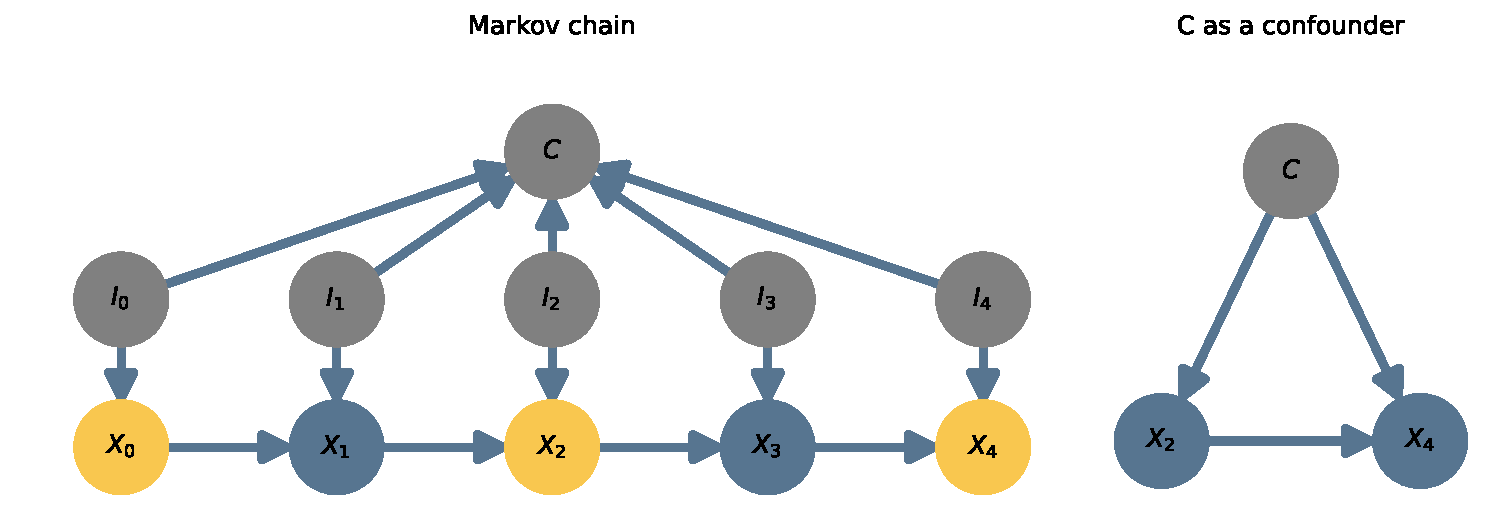
\includegraphics[width=\textwidth]{5origlcd_marginal.pdf}
    \caption{Graphical representation of the LCD context as constructed by \citet{versteeg2019boosting} applied to a Markov chain, and its marginalization over the three relevant variables.}
    \label{fig:5:origlcd}
\end{figure}
 

\subsubsection{Order-based Context Design}

We hypothesize that a more specific context is more effective. Given a variable pair $X,Y$, the original context makes a distinction whether there is an intervention anywhere in the system. Most of these interventions don't even affect $X$ or $Y$. We would like a context that makes a distinction between an environment with an intervention that affects $X$, and an envirenonment without such intervention. 

To construct a context based on this idea, we require two adaptations. First, for each variable $X$ we have a separate context variable $C_X$ that we use to test the relation $X\to Y$. Second, we need to estimate whether a given intervention is expected to affect $X$. 

The approach in this thesis is to estimate a causal order of the variables. Assuming acyclicity, interventions on genes later in the order than $X$ cannot affect it. Thus, we set the context to $1$ only if the intervention target is earlier in the order than $X$, or if $X$ is intervened on. 

Formally, we look at variable pairs $X_i, X_j$, and test the causal relation $X_i\to X_j$. For each variable $X_i$, we have some observation data points and intervention data points, such that $X_i = (X^O_i, X^I_i)$. The elements of the intervention data points $(X^I_i)_k$ are indexed according to the variable that is intervened on. For example, the intervention on $X_i$ itself is $(X^I_i)_i$. The inferred variable order is represented by a permutation $\pi$, such that $\pi_i$ indicates the position of variable $i$. We now construct the context $C_{X_i} = (C^O_{X_i}, C^I_{X_i})$ as follows.

$$\begin{array}{ll}
(C^O_{X_i})_k & =0 \\
(C^I_{X_i})_k & = \begin{cases}
    1 \text{ if } \pi_k\leq \pi_i \\
    0 \text{ if } \pi_k> \pi_i    
\end{cases}
\end{array}$$

Before we move to the experiments detailed in the next chapter, there is one problem that remains to be tackled. When we wish to predict the effects of variable $X_i$, we cannot use the intervention data point in which $X_i$ is intervened on. In fact, we use this data point to evaluate our prediction. However, the order inference algorithm requires this data to determine the position of $X_i$ in the order. Therefore, we can only use this algorithm to infer the order of the other variables $X_{\backslash i}$, and need a separate algorithm to infer the position of $X_i$.

\subsection{Estimating Variable Position in an Order}

Given the order of variables $X_{\backslash i}$, we wish to estimate the position of variable $X_i$. For this task we may use all intervention data, except the effects of the intervention on $X_i$. Some useful information may be found in the effects of the other variables on $X_i$. The intuition is that variables that significantly affect $X_i$, should be earlier in the order. 

We need to determine when we consider these effects to be significant. We construct a binary ground-truth in the same way as before, by subjecting the intervention table to a threshold. However, since the task is different we may choose a different threshold. We decide on the threshold using a simple analysis.

The task of estimating the position of a variable $X_i$ is not trivially defined. In our analysis, we first infer the order including $X_i$. We then remove it from the order and use the available data to estimate its position again. This allows us to evaluate the estimated position by comparing it to its original position. Note that the order of the remaining variables could be different if we would infer it without including $X_i$. However, we assume that the influence of including $X_i$ is minimal on the order of all other variables. 

The algorithm works as follows. We apply a threshold $T$ to the absolute values of the intervention table $\B{X} \in \mathbb{R}^{N\times N}$. Like before, $\B{X}_{ij}$ is the relative expression level of gene $i$ in the experiment with gene $j$ knocked out. This yields a binary ground-truth of significant effects of each intervention. For each $X_i$, we look up which interventions affect it significantly according to this ground-truth. Using the inferred order $\pi$, we find the position of the latest significant cause of $X$. The estimate of the position of $X_i$ in this order is directly after this latest cause. This way, all significant causes are earlier in the order.

\begin{figure}[]
    \centering
    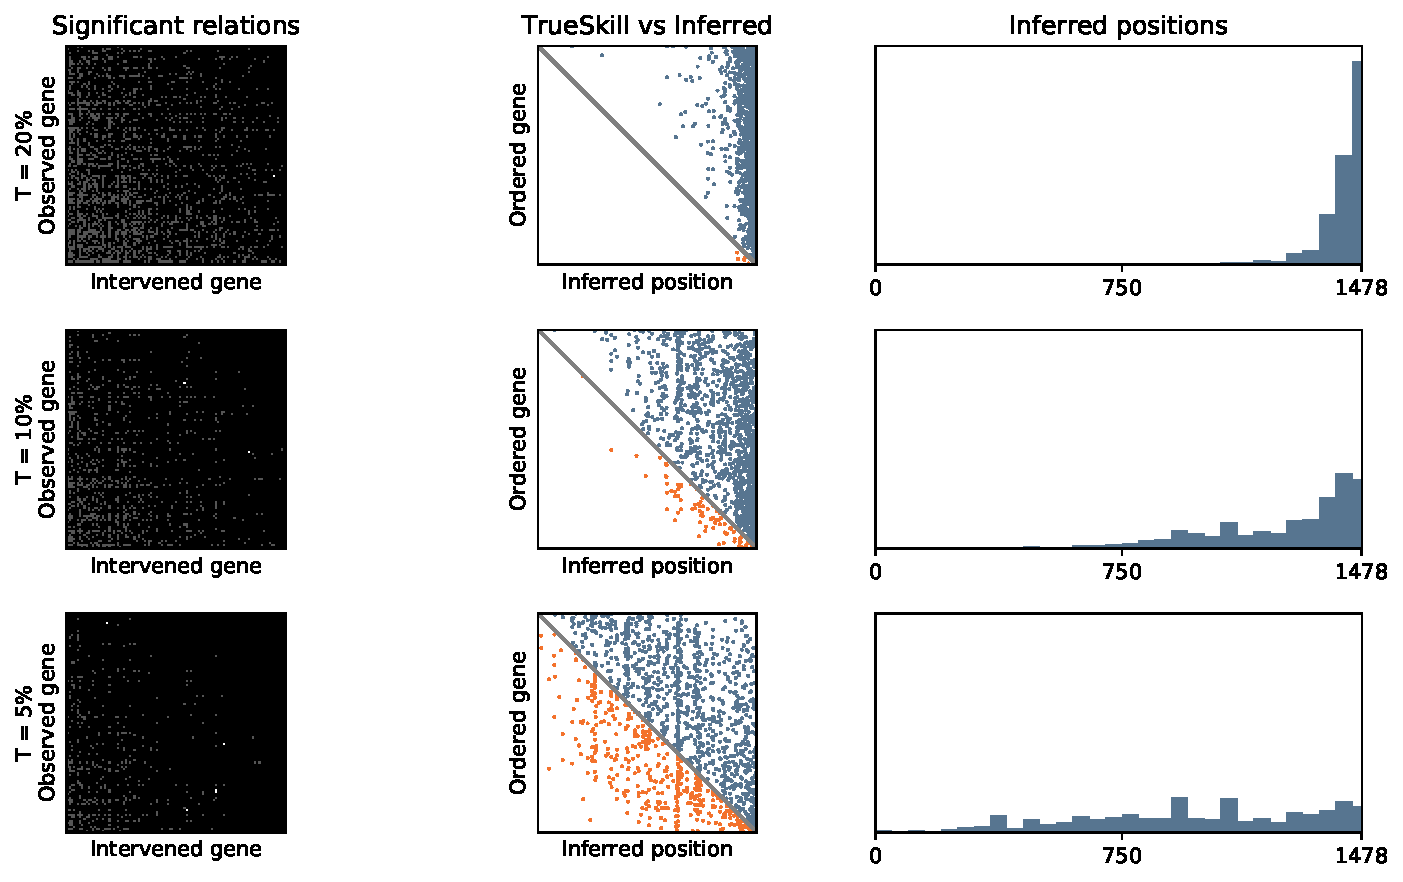
\includegraphics[width=\textwidth]{5inferred_positions.pdf}
    \caption{Analysis of test gene position inference for three different thresholds on the absolute expression values.}
    \label{fig:5:positions}
\end{figure}

Figure \ref{fig:5:positions} shows the results of the analysis for ground-truth thresholds $5\%$, $10\%$, and $20\%$. The left column shows the significant relations given the threshold, where the variables are ordered by the inferred order. Visually, for each gene on the rows, we look up the significant relation furthest to the right. The middle column shows only these last relations, and thus the estimated position for each gene. Note that if the order were correct, and no other order was possible (e.g. if the variables were on a Markov chain), the perfect positions would follow the gray diagonal line. Orange positions are estimated earlier in the order, blue positions later. The right column shows the distribution of estimated positions. 

% We choose threshold $10\%$ for our experiments. 
Threshold $5\%$ yields the nicest distribution of estimated positions. Many variables are placed at early positions compared to the results for higher thresholds. However, many of these early positions are earlier than their true position in the inferred order. This is not necessarily wrong, but we cannot verify this. If we make a lot of mistakes, the context becomes meaningless. We do not want to risk this. On the other hand, threshold $20\%$ estimates most positions to be far in the order. This means we approach the original context definition, since most interventions will be earlier than the estimated position of most genes. We choose threshold $10\%$ for our experiments as a good middle way.











% - How does the LCD method generally work?
%     - Why is it chosen? How does it generally perform? What is expected of it?
%     - On what assumptions does it rely?
%     - How is it proven?
%     - What statistical test is used?
% - How are the order-based and original context variables constructed?
%     - The puzzle of context construction
%     - Original C, graphical problem
%     - Order-based C, (still problematic?)
%     - Introduction to the problem of placing test genes in an order of train genes
%     - How is position inferred?
%     - Short analysis, justification of value threshold parameter
%     * something about 'detail', see notes Joris

% Somewhere:
% - L2 boosting preselection for speedup and great baseline (although not as good in other papers)

% Maybe:
% Note that the discrete nature of the variables and their relations makes the question of exogeneity nontrivial, and we do not provide any proofs here.

% \subsection{Local Causal Discovery}

% Local Causal Discovery has been proposed as a fast, incomplete algorithm to discover ancestral relations. The original formulation by \citet{cooper1997simple} depends on an underlying Bayesian Network and thus acyclicity. A more recent formulation by \citet{mooij2016joint} generalizes the algorithm to SCMs that allow cycles. 



% \subsubsection{Assumptions}

% The algorithm tests for a causal relation $X\to Y$ between two endogenous variables, using a third exogenous variable $C$ (the context). A small set of statistical independence tests restricts the set of possible causal subgraphs with $X$, $Y$ and $C$, and allowes us to infer under some circumstances that $X$ is an ancestor of $Y$. 

% LCD is based on the following assumptions:

% \begin{enumerate}
%     \item Underlying SCM (JCI-0)
%     \item Exogeneity of a context variable (JCI-1)
%     \item Causal faithfulness
%     \item Unbiased data selection
%     \item Independence oracle, and Dependence oracle
% \end{enumerate}



% \subsubsection{Statistical tests}

% LCD specifically discovers those causal relations, which effect can be measured from the data as $\Prb _M(Y|do(X=x)) = \Prb _M(Y|X=x)$. This is the case when only $X$ has an effect on $Y$ (i.e. no confounding or effect from $C$). Figure \ref{fig:5:lcdgraphs} shows the three subgraphs that satisfy this condition. Note that all possible relations between $C$ and $X$ given the exogeneity assumption are included.

% All subgraphs satisfy one independence and five dependence relations:

% \begin{enumerate}
%     \item $C \CI Y \given X $
%     \item $C \nCI X$
%     \item $X \nCI Y$
%     \item $C \nCI Y$ (follows from 2 and 3)
%     \item $X \nCI Y \given C$ (follows from 1 and 3)
%     \item $C \nCI X \given Y$ (follows from 1 and 2)
% \end{enumerate}

% The last three relations can be infered from the first three, using the causal faithfulness assumption and the Markov property. \citet{cooper1997simple} proved that the first three relations are sufficient to infer the causal relation $X\to Y$, by enlisting all possible subgraphs. 

% Most LCD implementations only check the first three relations. However, if assumptions are violated, some nonexistent causal relations might be infered. One can sacrifice recall for precision by testing some or all of the last three relations. \citet{cooper1997simple} warns specifically that the independence relation ($C \CI Y \given X$) is vulnerable to faithfulness violations, and suggests testing the fourth relation ($C \nCI Y$) as well. \citet{triantafillou2017predicting} aim for high precision and test all six relations.

% A common choice of dependence test is the two-tailed Fisher z-test \citep{fisher1924distribution}, which tests if the partial correlation is zero. Specifically, if we want to test $X \nCI Y \given Z$, we set the hypotheses:

% \begin{itemize}
%     \item[$H_0$:] $\rho_{XY|Z}=0$
%     \item[$H_A$:] $\rho_{XY|Z}\not = 0$
% \end{itemize}

% The partial correlation 

% z-transform -> test statistic z

% test hypothesis: p = 2*PHI(-sqrt... |z|)

% Pragmatic: use as independence test as well (different alpha, usually same value, but e.g. not in \citet{triantafillou2017predicting})


% SOMETHING ABOUT ASYMMETRY, but what was it and where did I read it?


% 6 pages

\newpage
\section{Experiments}
\label{chapter:experiments}

% SECTIONS
% Experimental design (like LCD, e.g. preselection)
% Metrics

\subsection{Experimental Set-up}

The \citet{kemmeren2014large} dataset contains the expression levels of 6.182 genes in 262 observation experiments, and as a result of 1.479 knock-out experiments. We describe this dataset as $\C{D}=(\B{O}, \B{X})$ with observation data $\B{O} \in \mathbb{R}^{6182\times 262}$ and intervention data $\B{X} \in \mathbb{R}^{6182\times 1479}$. $\B{O}_{ij}$ is the relative expression level of gene $i$ in the $j$-th observation, $\B{X}_{ij}$ is the relative expression level of gene $i$ in the experiment with gene $j$ knocked out. If we select only the intervention effects on genes that were also object of a knock-out experiment, we are left with the intervention table $\B{X}^I \in \mathbb{R}^{1479\times 1479}$.

\subsubsection{Data Folds and Bootstrapping}

The task is to predict per knock-out which genes are significantly affected, using the intervention data of the other knock-outs and the observation data. A leave-one-out experimental set-up would use all this data. Since variable preselection and order inference are time consuming, we choose a 5-fold train-test split set-up instead. The effects of each knock-out in a test fold are inferred from the remaining four train folds. In the spirit of this set-up, we also split the observational data, such that there is some variation in the observation data used per test fold.

From previous work on this dataset such as that of \citet{versteeg2019boosting} we know that only the most stable predictions may beat the baselines. We therefore apply the same bootstrapping method. We subsample the train data 100 times,  sampling 50\% without replacement. The predictions inferred on the subsamples are aggregated, allowing us to sort the predictions by confidence. 

We compare two methods of aggregating predictions. A \textit{discrete prediction} counts the number of times a relation was predicted, thus yielding a score between 0 and 100. A \textit{continuous prediction} estimates the confidence per prediction using the necessary condition of LCD that $C\CI Y$. The score is the sum of $-\log p_{C\CI Y}$.

\subsubsection{Evaluation}

The intervention data is transformed to obtain a score that indicates the significance of the causal relation. In evaluation, a certain percentage of highest scoring relations is taken as \textbf{ground-truth}. 

We compare two transformations of the intervention data to score the significance of each relation. The \textit{standardized score} $\B{S^S}\in \mathbb{R}^{6182\times 1479}$ is taken directly from the work of \citet{versteeg2019boosting}, such that we can directly compare our results. The effects on gene $j$ are normalized using the empirical mean and standard deviation of that gene in the observational data. The absolute value is taken to consider both upregulation and downregulation:

$$
S^S_{ij}=\frac{|X_{ij}-\mu_j|}{\sigma_j}
$$

This score prioritizes that every gene should occur as an effect in any ground-truth set, when it is possible that some genes never occur as a cause.

A large standard deviation in the expression of some gene is likely to mean that the gene is significantly affected by many other genes. We introduce a simpler \textit{absolute score} that does not imply a prioritization of including all genes as an effect. This is the same score used in the order-based LCD algorithm:

$$
S^A_{ij}=|X_{ij}|
$$

Furthermore, we consider two \textbf{filters} on the set of predictions. \citet{kemmeren2014large} mention that the knock-out genes were selected based on their role in regulating gene expression. This implicates that the group of knock-out genes differs qualitatively from the remaining genes. Therefore, we consider a filter of only effects on those genes. 

For the second filter we use the inferred order and test gene position. We only evaluate relations that explicitly comply to the inferred order and position. Note first that this leaves only a small number of ground-truth relations, since the distribution of inferred positions is skewed to the right, having relatively little candidate descendants. This second filter might provide some insights on the performance on those causal relations that our LCD algorithm is most explicitly concerned with.

\subsection{Method Implementation}
% L2-boosting
% Order inference, position inference, LCD (adaptation of Versteeg) (discarding relations due to indep. test)
% Baselines: ICP, original LCD, L2-boosting, random

The order-based LCD algorithm is implemented as an adaptation of the LCD algorithm by \citet{versteeg2019boosting}. Where they use the original context that distinguishes between observation and intervention data, we insert our order and position inference algorithms to construct an order-based context for each test variable. We compare our results to the same baselines used in their paper. The method implementation and baselines are shortly discussed here. 

All methods start with variable preselection by L$_2$-boosting \citep{schapire1998boosting}. This preselection saves significant computation time. It works so well, that it is taken as a baseline method. \citet{versteeg2019boosting} show that performance of LCD is improved when this preselection is applied, so at least for the strongest predictions we do not sacrifice performance.

L$_2$-boosting selects at most 8 test variables that are most predictive for each effect variable, using the joint observation and intervention data. For LCD testing a relation $X\to Y$, this means that at most 8 causes $X$ from the test split are considered for each effect $Y$. L$_2$-boosting iteratively applies least squares regression to the residuals, eliminating variables that are least predictive. 

To compute the order-based context, our LCD algorithm first infers an order on the variables in the train split using TrueSkill. Next, the position of each gene $X$ in the test split is individually estimated. From the order and the gene position a context $C_X$ is computed and the relation $X\to Y$ is tested for all $Y$'s of which $X$ is a preselected variable. 

For comparison, we show the LCD and ICP results from \citet{versteeg2019boosting} that use the mean-variance test and L$_2$-boosting. Their L$_2$-boosting baseline results are also shown. Note that we evaluate these results not only on their standardized ground-truth score, but also on an absolute score, resulting in somewhat different graphs.
% 5 pages

\newpage
\section{Results and Analysis}

% SECTIONS
% Results

% Analysis
% What the hell is going on? Why are the strongest results in violation of the order? (Is the order interpreted in the wrong direction?...)

% Ablation study, Sensibility analysis of hyperparameters
% Weaknesses (in relation to assumptions)

% Selecting only compliant relations: there's just very few left, they happen to be wrong?


% ROCs
We evaluate the methods using receiver operating characteristic (ROC) curves. The methods assign a score to every causal relation. The ROC curves plot how the number of true positives and false positives change for different thresholds on this score. Each method only assigns a score to some relations. If we require predictions beyond this point, we can only guess randomly. 

The ROC curves in Figure \ref{fig:7:rocshort} are discussed in detail in this section. For each method, we aggregated continuous predictions and evaluated on the absolute score ground-truth. The curves for other settings are shown in Appendix \textbf{APPENDIX}. The conclusions that we draw here are applicable to the other settings as well. 

ROC curves show the number of true positives on the x-axis versus false positives on the y-axis. Good methods rise quickly. Figure \ref{fig:7:rocshort} shows different ways to evaluate the same methods. Each column represents a different ground-truth threshold. This threshold indicates the percentage of top scoring relations that are considered to be true. Each row represents an evaluation filter. Methods are evaluated on the full dataset, the intervention table, and the relations that are explicitly compliant to the inferred order and test variable position. After the last prediction of a method, we indicate random guessing with a dashed line.

We first recapitulate the main findings of \citet{versteeg2019boosting} about the baseline methods. Then we compare order-based LCD to them. Finally we discuss the effect of preselection to our method.

\begin{figure}[h]
    \centering
    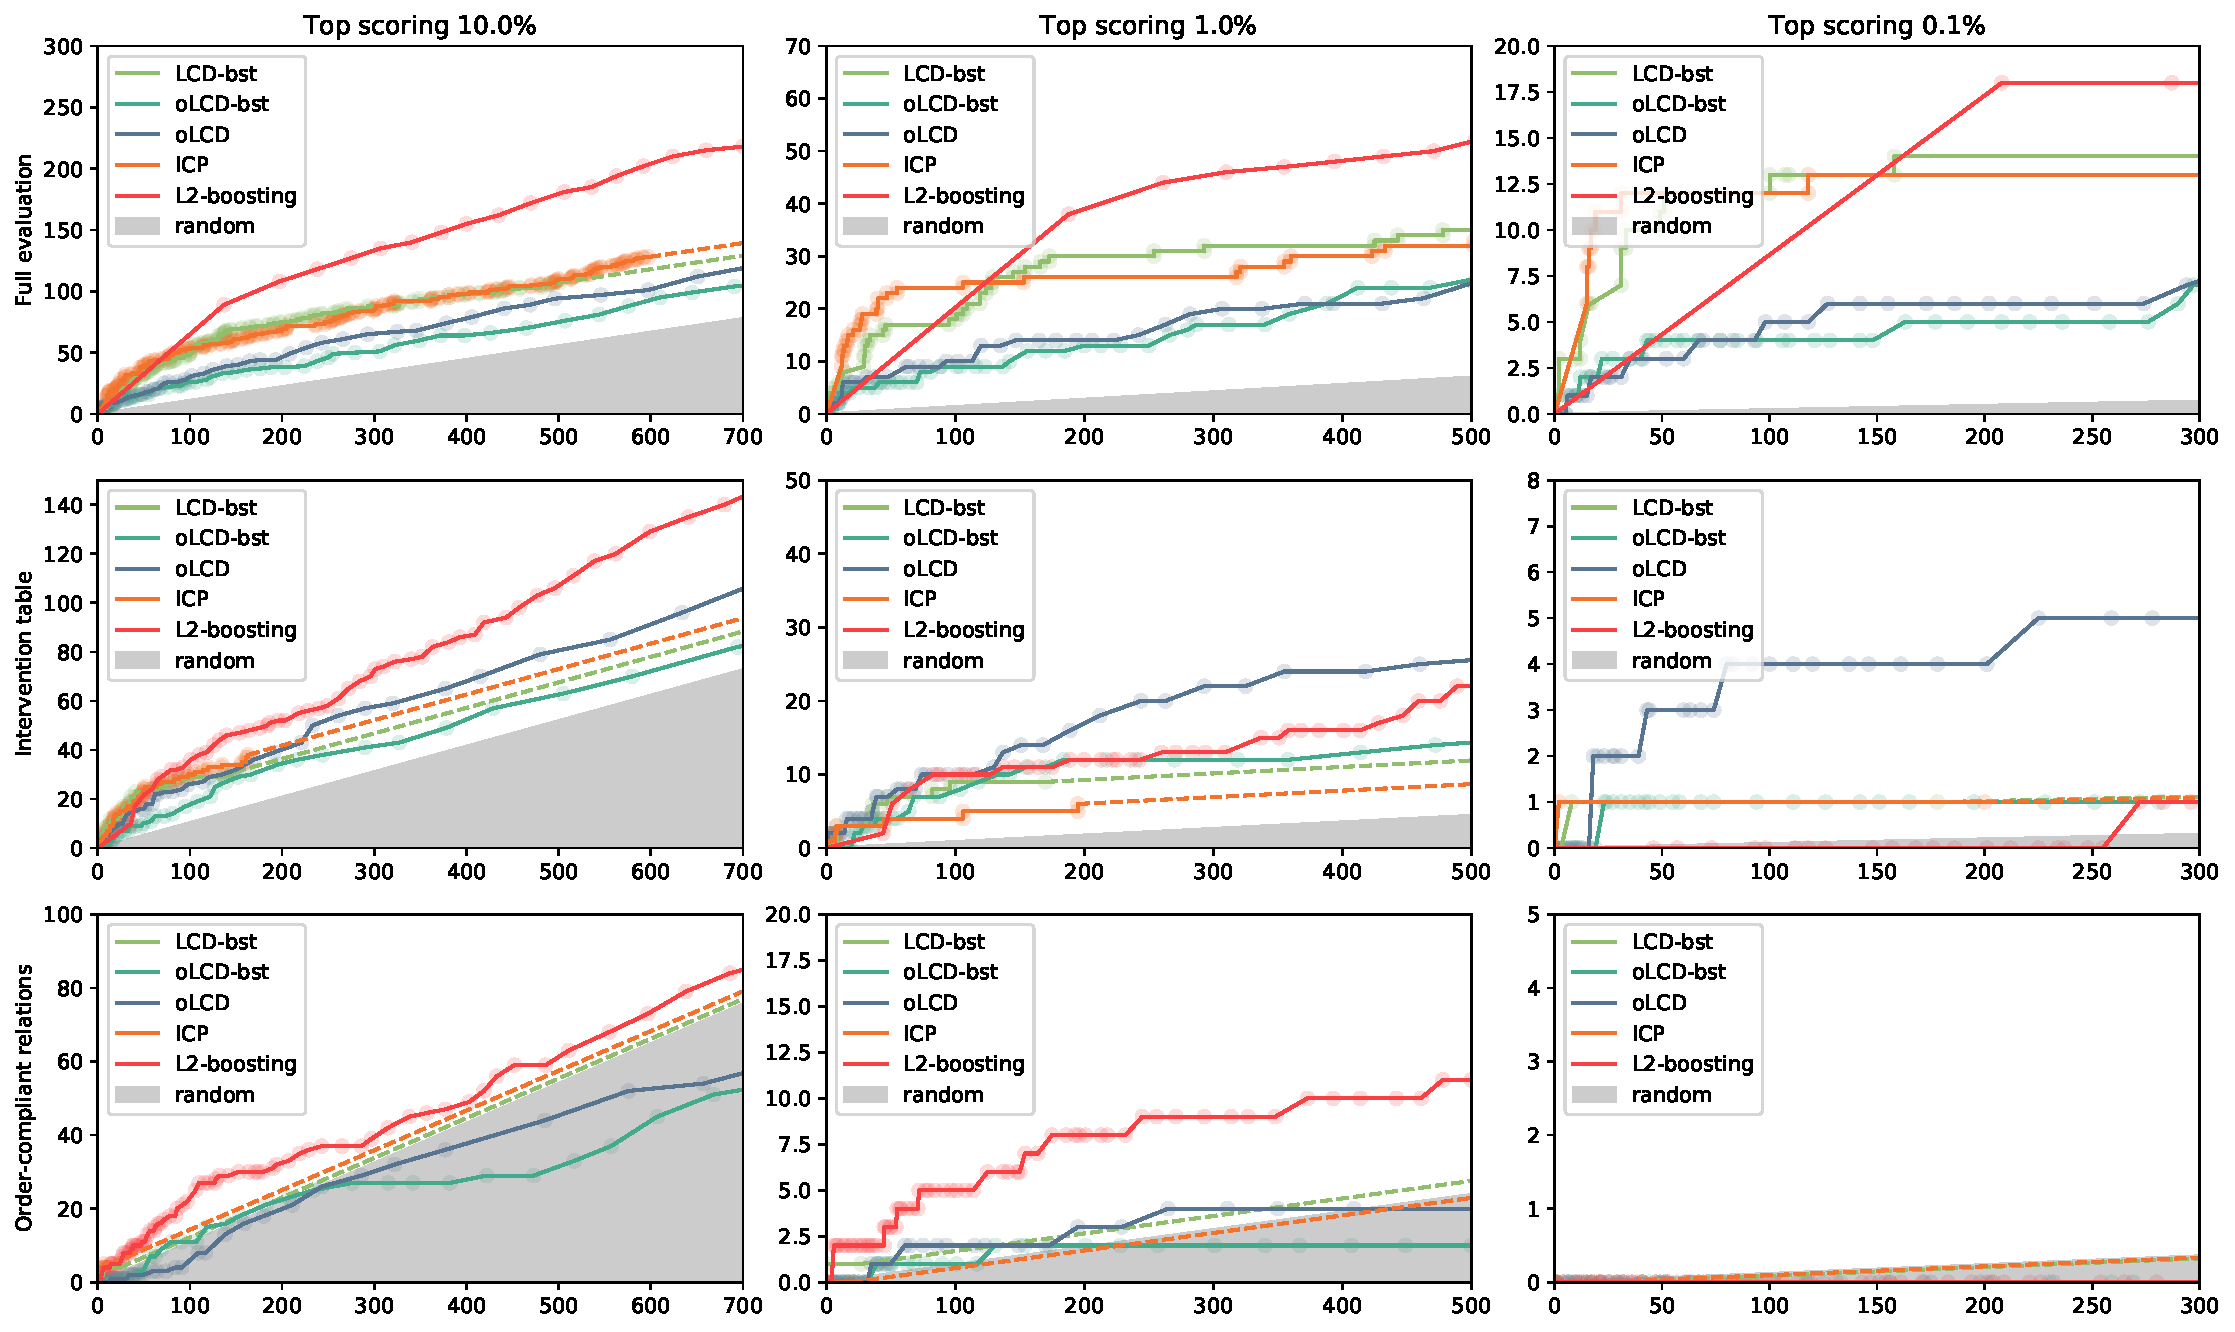
\includegraphics[width=\textwidth]{ROC_filter_threshold_absgt_scorespred_short.pdf}
    \caption{Partial ROC curve using the absolute ground-truth with aggregation of continuous scores.}
    \label{fig:7:rocshort}
\end{figure}

\subsubsection{Baselines}

% ICP/LCD is more fine-grained at start
Since we compare order-based LCD to the baseline methods of \citet{versteeg2019boosting}, we first summarize their findings\footnote{The exact ROC curves of that paper can be found in Appendix \textbf{APPENDIX}, in the top row of Figure \textbf{FIGURE}}. 226 relations are predicted in all subsamples by the non-causal L$_2$-boosting baseline. They are shown as the first point in the ROC curves. When we wish to use this method to make fewer predictions, we can only guess randomly within this set. The predictions of ICP and LCD are more fine-grained, because their 200 strongest predictions contain multiple confidence levels. LCD and ICP have many more true positives in their top 70 than L$_2$-boosting, as can be seen in the top row of Figure \ref{fig:7:rocshort}. This is where the non-causal baseline is beaten.

% LCD is largely explained by L2
Moreover, \citet{versteeg2019boosting} investigate the impact of L$_2$-boosting preselection on LCD. Preselection improves the method significantly. Preselection is what makes LCD comparable to ICP, being computationally less expensive. LCD can be interpreted as a causal filter on the non-causal L$_2$-boosting baseline. The baseline works surprisingly well on its own. The LCD conditions are a causal check that filter out mistakes of in the baseline, specifically causation in the opposite direction and confounding.

% LCD does not make many predictions
As a last remark, we note that LCD with preselection does not make many predictions. Only 608 relations of 126.103 preselected relations are assigned a non-zero score. When we are interested in beating the L$_2$-boosting baseline, this does not matter. The baseline is only beaten in the first 70 predictions. However, if we want to select a large number of relations, this is a restriction.


\subsubsection{Order-based LCD}

% Direct comparison: worse
Order-based LCD performs significantly worse than the baselines when evaluated on the full data set. The strongest predictions contain more false positives than LCD and ICP. 

Better results can be seen when we evaluate on the intervention table. Order-based LCD beats the non-causal baseline in the strongest predictions, and stays comparable after that. LCD and ICP perform slightly worse. 

When we only evaluate on relations that explicitly comply to the inferred order, order-based LCD does not perform better than LCD or ICP. This is unexpected, since the order-based context should be most informative for these relations. Instead, comparing to the results on the intervention table, it seems like the performance is better on relations that violate the order.

What is most important to the causal inference, is that the data points in which a true ancestor is intervened on, are associated with context value 1. Many of the remaining context values should be 0, such that the two clusters can be distinguished and the causal relation can be identified. Since the number of true ancestors may not be large, we are allowed to make many mistakes in the context.

% positions are skewed to the back
Position inference is constructed such that the positions generally tend to be estimated later in the order than they actually are. Therefore, what may seem like an order violation may just be a conservative estimate of the position.

% 'wrong order' does not create wrong prediction; order and position is messy
More importantly, the order inference and position inference algorithms are far from perfect. Many relations that are taken as order violation may be compliant to the real order in the underlying graph. Although a messier order and position reduces recall, it is not necessarily harmful to the precision. The context may not be very informative of the order, it still satisfies the exogeneity assumption. The LCD conditions imply an ancestral relation regardless of the interpretation of the context values. Still, a more informative context is desirable, since we expect LCD to be able to detect more of the true relations.


% Boosting bad
\subsubsection{Preselection}
Contrary to the results of the original LCD algorithm, L$_2$-boosting preselection does not have a clear benefit to order-based LCD. In fact, in the evaluation on the intervention table it reduces performance. 

We can interpret the boosting baseline as a filter on LCD. In the case of the intervention table evaluation, this filter takes out true strong predictions, indicating that order-based LCD uses information that is not found at all by the non-causal baseline. This interpretation is the reverse from that of \citet{versteeg2019boosting}, who interpret LCD as a filter on L$_2$-boosting that uses causal information to select the strongest relations beating boosting in the first predictions. 


% More predictions, some information about top 1000+? Some causal info not in L2?




% If accidentily right, still predicts right (accidentilly wrong, doesn't predict)
% What is actually relevant according to the hypothesis: interventions on ancestors should be in cluster C=1, many of the remainder should be in C=0. This can still be the case when order and position are messy, especially when the graph is sparse and there aren't many ancestors.

% Int filter: unfair comparison

% Comparable to L2 further on, without requiring it as preselection. (much further, on int data, even better without boosting)




% - Versteeg improves within the strongest prediction of L2: 226 relations are predicted in all subsamples; large part explained by L2 -> here it doesnt really matter
% - We present results of one setting (abs, cont) here, results of this setting of normal LCD are comparable to their setting (std, disc). We shortly discuss differences in the end.
% - LCD is a filter on L2-boosting
% - normal LCD does not predict much, but its strongest predictions are better than just taking L2
% - orderLCD makes more predictions (see wider ROCs in appendix). The weaker predictions are better than LCD which has to resort to random guessing. Worse than L2, so not that useful in itself but interesting direction of research.
% - orderLCD only improves over L2 in two settings
% - boosting doesn't help, and is harmful on intervention table evaluation!

% The intervention table contains the relations in explicit violation of the order (inferred position is later than target in order), relations explicitly complying to the order (inferred position is earlier than target in order), and relations for which the compliance is unknown (target is also in test split). Compared to the results on the intervention table, it may seem like order-based LCD performs better on explicit order violations than on compliant relations. 

% Versteeg: top 20 is pretty good, deBoer: top 400 is bad but comparable to baseline



% 12 pages

% \newpage\phantom{blabla}
\newpage
\section{Conclusion and Outlook}
\label{chapter:conclusion}

% SECTION
% Impact of results
% Next steps in this direction
% Future of causality field

% IMPORTANT: it was a very hard problem, high dimensionality and little data, no true labels, complex system


% What did we do? ("limited success")
After a decade that has shown unbelievable successes of statistical AI, purely statistical methods are reaching limits. This warrants a revaluation of symbolic AI, and sparks new interest in the interface of the two schools. Causality arises as a field with the ambitious goal to unveil cause-effect relations with a combination of deduction from datasets and induction from background knowledge. 

We took a dataset of gene perturbation experiments and investigated an adaptation of LCD to discover causal relations between genes. Since we found that there was only limited feedback, we hypothesized that a causal order could inform the LCD context variable. 

An extensive analysis of methods to estimate variable order from the data showed TrueSkill to be the most effective option. A straightforward method was then analysed to infer the position of a tested gene in the order. Finally, the order was used to construct a context variable for LCD, and order-based LCD was compared to baseline methods.


% Contributions
\subsection{Contributions}
The main contributions of this thesis are listed below.

\setlist{nolistsep}
\begin{itemize}[noitemsep]
    \item A metric was introduced to evaluate the task of estimating variable order.
    \item Statistical properties of the \citet{kemmeren2014large} dataset were analysed, which can be used to inform causal discovery methods.
    \item Order estimation methods were thoroughly analysed on the \citet{kemmeren2014large} dataset.
    \item An order-based LCD method was introduced and shown to use information that is not used by the non-causal regression-based baseline
\end{itemize}


% Suggestions for Future Work
\subsection{Suggestions for Future Work}
The results of this thesis show the potential of using variable order for causal discovery. This opens up some interesting directions for further research.

\setlist{nolistsep}
\begin{itemize}
    \item The estimate of variable order is derived from the data, and used to construct context variables. This raises the question to what extent the exogeneity assumption is threatened. Given a certain method of order inference, what functional forms of the context variable are allowed?
    \item Experiments on a wide variety of generated datasets would provide useful insights about the properties of order-based LCD. For example, does it work better on sparse SCMs? How harmful are cycles?
    \item Generalizations to datasets with more datapoints per intervention, or to other inference methods like ICP would be very interesting. 
\end{itemize}

Brainstorm:
- Throw out more interventions to make it more distinct from original LCD
- Define a new task to predict the deviation, e.g. select C=1 from interventions such that linear regression on C=1 yields a good estimate (are we allowed to evaluate like this, or are we using the train data?)
- Look further into order inference: use the continuous scores (e.g. TrueSkill adaptation), infer partial orders more in line with the underlying data, ...
- Improve position inference: maybe find order and position jointly (find an order specific to each cause gene? Select genes likely to be ancestor in other way)
- Test further: Apply order-based context to ICP (or other context-based methods); apply to different datasets with different properties
- Broaden scope: Investigate how to incorporate the knowledge of intervention target in a more fine-grained manner
- Experiment with different (more fine-grained?) ways to construct a context. Drop the order, keep the same intuition and directly remove the X-center of the intervention data.


% \item order is based for a large part on data values. Is the dependence of the order on the data confuscated enough to make the exogeneity assumption valid? Theoretical analysis of the allowed functional dependence of discrete exogenous variables on data.
% \item filter on intervention table, these genes were selected as knock-out for a reason, maybe its an easier task? It is definitely a different task.
% \item predicting continuous values could be a better task
% 2 pages

\newpage
\bibliography{references}

\appendix

\newpage
\section*{Appendix A}

\end{document}
